\chapter{Single-photon nonlinearities in two-mode optomechanics}
\label{ch:Komar2013}
%From \cite{Komar2013}
%%%%%%%%%%%%%%%%%%%%%%%%%%%%%%%%%%%%%%%%%%%%%%%%


%%%%%%%%%%%%%%%%%%%%%%%%%%%%%%%%%%%%%%%%
%%%%%%%%%%%%%%%%%%%%%%%%%%%%%%%%%%%%%%%%
\section{Introduction}
Optomechanical systems (OMSs) involve the interaction between optical and mechanical
modes arising from 
%the 
radiation pressure force, canonically in an optical
cavity with a movable mirror \cite{Kippenberg2008,
Marquardt2009, AspelmeyerNJP2008, Genes2009, Favero2009}.
Recent progress in optomechanical (OM) cooling techniques
has been rapid \cite{Metzger2004, Gigan2006, Arcizet2006, Kleckner2006,
Corbitt2007, Schliesser2008,Thompson2008,Wilson2009}, 
%\cite{Metzger2004, Gigan2006, Arcizet2006, Kleckner2006,
%Corbitt2007, Schliesser2008,Wilson2009,Groblacher2009, Jayich2008,
%Thompson2008},
and 
experiments have now demonstrated cooling to the
mechanical ground state
% KS: Shouldn't one cite Chan2011, Teufel2011, and O'Connell2010 ? 
% KS: I admit that the latter is slightly inappropriate here, but these are the three
% KS: ground-state experiments to date, right?
\cite{O'Connell2010,Teufel2011,Chan2011},
%\cite{Chan2011, Riviere2011, Safavi-Naeini2012, Teufel2011, O'Connell2010},
OM induced transparency \cite{Weis2010,Safavi-Naeini2011},
and coherent
photon-phonon conversion \cite{Fiore2011,Verhagen2011,Hill2012}.
These developments have
attracted significant interest, and
motivated proposals for applications
exploiting OM interactions at the quantum level,
ranging  from
quantum   
 transducers  
 \cite{Stannigel2010,Safavi-Naeini2011a,Regal2011,Taylor2011}
 and mechanical storage of light \cite{Zhang2003, Akram2010,Chang2011}
 to single-photon sources \cite{Rabl2011} and OM quantum information processing 
 \cite{Stannigel2012,Schmidt2012}.
 %\cite{Safavi-Naeini2011a, Stannigel2011, Stannigel2010,Zhang2003, Akram2010}
%  and routers
% % KS: I think the paper by Heinrich2011 does not discuss routing, so I would
% % take it out here
%   \cite{Stannigel2012} to single-photon sources
%  \cite{Rabl2011,Nunnenkamp2011} and mechanical 
%  storage of light
% \cite{Chang2011}.
Significant advantages of OM platforms for these 
applications are
 the possibility for mass production and on-chip integration using
 nanofabrication  technologies, %\cite{Gavartin2012, Krause2012}
 wide tuneability 
 %\cite{Sankey2010} 
 and the versatility of mechanical oscillators 
 to
 couple to a wide variety of quantum systems \cite{Schoelkopf2008}.
% KS: We should give some hybrid-references here: spins, quantum dots, sc qubits, atoms 
% KS: Is there a good overview? @PR, what about the hybrid book-chapter?
% KS: Otherwise we would have to cite individual references for each system.
 
 
The force exerted by a single photon on a macroscopic
object is typically weak; consequently,
experiments have so far 
focused on the regime of strong optical driving, where
the OM interaction
is strongly enhanced but effectively linear
\cite{Groblacher2009,Teufel2011a}
%\cite{Marquardt2007,Wilson-Rae2007,Dobrindt2008}.
% KS: I think we should change this to either an experimental reference or to
% KS: a review article like [1-3]. The cooling-references somehow seem a bit
% KS: strange here.
% SB: reason for these: early linearized quantum theory of OM.
% SB: we agree these refs should be shuffled
However, recent progress in the design of nanoscale OMSs
\cite{Chan2011,Eichenfield2009, Carmon2007, Ding2011}
%\cite{Eichenfield2009, Safavi-Naeini2012, Carmon2007, Ding2011}
and OM experiments in
cold atomic systems 
\cite{Gupta2007, Brennecke2008} 
% KS: The atomic OMS come a bit out of the blue. Maybe one can put them in a
% KS: separate sentence to make clear they are just a side remark. I think they
% KS: are never mentioned after this point, are they?
% SB: For now: leave this a sidenote and mention in Outlook.
suggests that the regime of single-photon 
strong coupling, where
the OM coupling strength $g$ exceeds the optical
cavity decay rate 
$\kappa$, is within reach of the
next generation of OM experiments.
In this regime, the inherently nonlinear OM interaction
is significant at the level of single photons and phonons~\cite{Marshall2003,
Ludwig2008, Rabl2011, Nunnenkamp2011}. 
For example, the presence of
a single photon can---via
the mechanical mode---strongly influence or even
block 
the transmission of a second photon, leading to
photon blockade.
This single-photon nonlinearity   was recently
analyzed for canonical OMSs consisting of a single
optical mode coupled to a mechanical mode 
\cite{Rabl2011,Kronwald2012,Liao2012}.
%\cite{Marshall2003, Ludwig2008, Rabl2011, Nunnenkamp2011}.
However, with a single optical mode, 
the OM coupling is highly off-resonant, 
leading to a
suppression of effective 
photon-photon interactions by the large mechanical
frequency $\omega_m \gg g$ \cite{Rabl2011}.
% KS: I put in PR's paper again, since this point is made more precise there


In this paper we develop a quantum theory of a weakly driven
\emph{two-mode} OMS
\cite{Miao2009, Stannigel2012,Ludwig2012, BasiriEsfahani2012} 
%\cite{Grudinin2010,Dobrindt2010, Miao2009, Cheung2011,Ludwig2012, Zhang2012}, 
in which two optical modes are coupled to
a mechanical mode. 
The key advantage of this approach is that
 photons in the two optical modes can be resonantly exchanged by absorbing or
 emitting a phonon via three-mode mixing.
 We extend our earlier results \cite{Stannigel2012}, where we discussed possible
 applications of resonant optomechanics such as single-photon sources and
 quantum gates,
 by exploring one-time and two-time photon correlations 
 of both optical modes.
 Specifically, we find that the photon-photon correlation function of the
 undriven optical mode exhibits delayed bunching for long delay times,
 arising from a heralded single mechanical excitation after detection of a
 photon in the undriven mode.
 Finally, we compare the two-mode OMS
 to the canonical atomic cavity QED system with 
 a similar low-energy level spectrum
 \cite{Carmichael1991, Brecha1999}.
% KS: I put 'canonical cQED' here, since one might otherwise think that we mean the atomic OMS  
 Despite several similarities we find that, 
 in stark contrast to the atom-cavity system, the OMS studied
 here does {\it not} exhibit nonclassical
 correlations unless the strict strong coupling condition $g >
 \kappa$ is met.
Our results serve as a guideline for OM experiments 
nearing the regime of 
single-photon nonlinearity, and for
potential quantum information processing applications
with photons and phonons.



The remainder of the paper is organized as follows. 
In
Sec.~\ref{sect:Multimode}, we introduce the system and details of the model.
In Sec.~\ref{sect:Averages}, we calculate the equal-time intensity correlation
functions of both  transmitted and  reflected photons, and discuss
signatures of nonclassical photon statistics.
In Sec.~\ref{sect:Delayed_coincidence}, 
we investigate two-time correlation functions
of the transmitted photons, and discuss delayed
coincidence correlations that indicate the heralded
preparation of a single phonon state.
Finally, we provide
a brief outlook on the feasibility of strong OM coupling 
in Sec.~\ref{sect:Experimental values}, 
and 
conclude
in Sec.~\ref{sect:Conclusion} with a summary of our
results.
Appendix \ref{sect:App:steady_state} contains details of our analytic model used to
derive several results discussed in the paper.



 
 
 
%%%%%%%%%%%%%%%%%%%%%%%%%%%%%%%%%%%%%%%%
%%%%%%%%%%%%%%%%%%%%%%%%%%%%%%%%%%%%%%%%
\section{Multimode optomechanics}
\label{sect:Multimode}
 
We consider the setup shown schematically in \reffig{fig:cartoon_a},
consisting of two optical cavities separated by a semitransparent mirror.  The cavity modes
are coupled by photons tunneling through the fixed mirror in the middle, and the
mode on the right couples to the motion of a vibrating endmirror %a mechanical
oscillator through radiation pressure.
% acting on the movable endmirror.
\begin{figure}
\centering
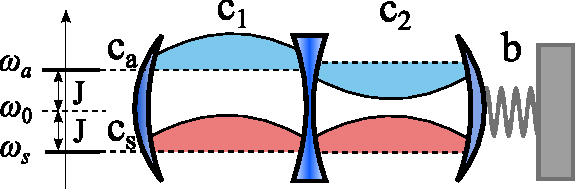
\includegraphics[width=0.65\textwidth]{./figs_Komar2013/fig1a.pdf}
\caption
[Two-mode optomechanical system]
{  
  \label{fig:cartoon_a}
  Optomechanical system consisting of
  two tunnel-coupled optical cavity modes
  $c_1$ and $c_2$, and a mechanical oscillator $b$ 
  coupled to one of the cavity
  modes by radiation pressure. 
  The coupled optical modes are diagonalized in terms of
  symmetric and antisymmetric modes, $c_s$ and $c_a$.
  }
\end{figure}
The Hamiltonian describing the system is $(\hbar=1)$
\bel
\begin{split}
\label{eq:Hamiltonian_0}
	H_0 =\; & \omega_0(c_1\+ c_1 + c_2\+ c_2) - J(c_1\+ c_2 + c_1\+ c_2)  \\
	& + \omega_m b\+ b -g(b\+ +	b)c_2\+ c_2  + H_{\text{dr}}(t),
\end{split}
\eel
where $c_{1,2}$ are annihilation operators for  the two
cavity modes, which we assume to be degenerate with frequency
$\omega_0$, and $J$ is the photon tunneling amplitude through the central
mirror. The motion of the endmirror on the right is described by a single
mechanical mode with annihilation operator $b$ and 
%resonant vibrational 
frequency
$\omega_m$, and the parametric
coupling strength $g$ corresponds to the shift of the
cavity frequency due to a single mechanical phonon. Finally,
$H_{\text{dr}}(t) = \sum_{i=1,2}\left( \Omega_i c_i e^{i\omega_L t}   +
\text{h.c.}\right)$ describes two coherent driving fields of amplitudes
$\Omega_i$ and frequency $\omega_L$, which are applied to the left and right
cavities. 


% % ==================================
% \begin{figure}[htb]
% \centering
% $\vcenter{\hbox{
% 	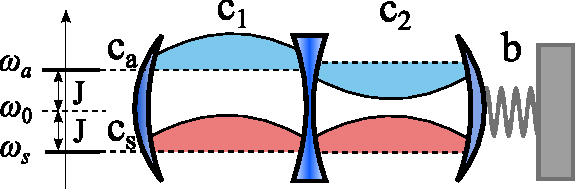
\includegraphics[width=0.48\textwidth]{./figs_Komar2013/fig1a.pdf}
% }}$
% 
% $\vcenter{\hbox{
% 	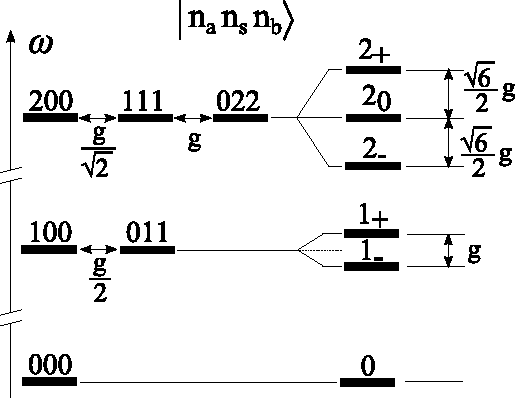
\includegraphics[width=0.48\textwidth]{./figs_Komar2013/fig1b.pdf}
% }}$
% \caption{ 
%   \label{fig:cartoon} (Color online)
%   (a)~Optomechanical system consisting of
%   two tunnel-coupled optical cavity modes
%   $c_1$ and $c_2$, and a mechanical oscillator $b$ 
%   coupled to one of the cavity
%   modes by radiation pressure. 
%   The coupled optical modes are diagonalized in terms of
%   symmetric and antisymmetric modes, $c_s$ and $c_a$.
%   (b) Level diagram showing  the  relevant  zero-, one- and two-photon states
%   at zero temperature and under the three-mode resonance condition
%   $\omega_s - \omega_a = \omega_m$. 
%   States are labeled by $\ket{n_a n_s n_b}$ denoting
%   the number $n_a$ ($n_s$) of antisymmetric
%   (symmetric) photons and the number of phonons $n_b$.
%    The optomechanical coupling $g$ splits
%    the degeneracy of states  $\ket{n_a n_s n_b}$ and
%   $\ket{n_a-1, n_s+1, n_b+1}$.}
% \end{figure}
% % ==================================




We are interested in a three-mode resonant interaction
in which the two optical modes exchange a photon
by absorbing or emitting a phonon in
the mechanical mode. 
We begin by diagonalizing
the optical part of $H_0$ in the first line of \refeq{eq:Hamiltonian_0}
in terms of the symmetric and antisymmetric combinations
of the optical modes, $c_s = \frac{1}{\sqrt{2}} (c_1 + c_2)$ and
$c_a = \frac{1}{\sqrt{2}}(c_1 - c_2)$, with 
eigenfrequencies  $\omega_{a,s} =
\omega_0 \pm J$. 
In the frame rotating at the laser frequency $\omega_L$ we obtain
\bel
\label{eq:Hamiltonian_tmp}
\begin{split}
	H' = &
	-\Delta c_a\+ c_a  
	- (\Delta + 2J) c_s\+ c_s + \omega_m b^\dag b \\
	&+ \frac{g}{2} 
	\left( c_a\+ c_s +  c_s\+ c_a \right) \left( b + b^\dagger \right)
	+ \sum_{\eta=s,a} \Omega_\eta (c_\eta^\dag +c_\eta),
	%+ \Omega_s (c_s^\dag + c_s),
\end{split}
\eel
where $\Delta = \omega_L - \omega_a$ is the laser detuning from 
the $c_a$ mode,
%$\delta_m=\omega_a - \omega_s-\omega_m$  
and $\Omega_{s,a}=(\Omega_1 \pm \Omega_2)/\sqrt{2}$. 
Next, we focus on the case of three-mode resonance,
$\omega_m = 2 J$, 
and assume $\omega_m\gg g,|\Delta|, \Omega_i$.
The third inequality here corresponds to 
a weak optical drive, the relevant limit for
studying  single-photon nonlinear effects in this work.
%  then this
%justifies neglecting the $\Omega_s$ term.
This   
%is fulfilled in experimental systems of interest  \cite{Grudinin2010, Zhang2012}, and 
allows us to make a rotating wave approximation
with respect to the remaining large frequency scale $\omega_m$, and  
in the frame defined by the
transformation
$U = \exp[- i\omega_m t (b\+b - c_s\+c_s)]$,  the Hamiltonian $H'$ simplifies to 
\bel
\label{eq:Hamiltonian_eff}
\begin{split}
	H = -\Delta (c_a\+ c_a+ c_s^\dag c_s) 
	+ \frac{g}{2}(c_a\+ c_s
	b + b\+ c_s\+ c_a)	+ \Omega_a (c_a^\dag + c_a).
\end{split}
\eel
This is the starting point for our analysis discussed below.
Note that the assumptions made in deriving Eq.~\eqref{eq:Hamiltonian_eff} are 
fulfilled in most experimental systems of interest  \cite{Grudinin2010, Zhang2012}, and
$H$  
%in Eq.~\eqref{eq:Hamiltonian_eff} 
represents a generic description for
resonant two-mode optomechanics \cite{Miao2009, Dobrindt2010, Cheung2011,
Ludwig2012}.

%In the following analysis we focus on the exact
%three-mode resonance, $\omega_m=2J$, 
%and assume that
%only the antisymmetric mode $c_a$ is externally driven, i.e.
%$\Omega_a\equiv\Omega$ and  $\Omega_s=0$. Then, by performing another unitary transformation, 
%$U = \exp[- i\omega_m t (b\+b - c_s\+c_s)]$, the system Hamiltonian simplifies to 
%\bel
%\label{eq:Hamiltonian_eff}
%\begin{split}
%	H = -\Delta (c_a\+ c_a+ c_s^\dag c_s) 
%	+ \frac{g}{2}(c_a\+ c_s
%	b + b\+ c_s\+ c_a)	+ \Omega_a (c_a^\dag + c_a),
%\end{split}
%\eel
%which we will use as a starting point for our analytic results discussed below.
%
%In the rotating
%frame defined by the transformation 
%%$H\rightarrow UHU\+$, where
%$U = \exp[-i\omega_L t (c_a\+ c_a + c_s\+ c_s) - i\omega_m t (b\+b - c_s\+
%c_s)]$,
%%and within the rotating wave approximation,
%the effective Hamiltonian is
%\bel
%\label{eq:Hamiltonian_eff}
%\begin{split}
%	H = 
%	-\Delta c_a\+ c_a  
%	- (\Delta + \delta_m) c_s\+ c_s 
%	+ \frac{g}{2}(c_a\+ c_s
%	b + b\+ c_s\+ c_a) \\
%	+ \Omega_a (c_a^\dag +c_a),
%%	+ \Omega_s (c_s^\dag + c_s),
%\end{split}
%\eel
%where $\Delta = \omega_L - \omega_a$ is the laser detuning from 
%the $c_a$ mode,
%$\delta_m=\omega_a - \omega_s-\omega_m$  
%is the detuning from three-mode
%resonance, and $\Omega_{a}=(\Omega_1 - \Omega_2)/\sqrt{2}$.
%% In the following analysis we are primarily interested in the case
%% $\delta_m=0$.
%In deriving
%Eq.~\eqref{eq:Hamiltonian_eff} we made a rotating wave approximation
%(RWA)
%in the large mechanical
%frequency, requiring  $\omega_m \sim 2J \gg \Delta,g,\delta_m$. 
%This condition is fulfilled in
%experimental systems of interest  \cite{Grudinin2010, Zhang2012}, and
%$H$ in Eq.~\eqref{eq:Hamiltonian_eff} represents a generic description for
%resonant two-mode optomechanics \cite{Miao2009, Dobrindt2010, Cheung2011,
%Ludwig2012}.
%Note that by choosing to drive near resonance with the antisymmetric mode,
%the drive is far off-resonant with the symmetric mode.
%As a result  the term
%$\Omega_s (c_s^\dag e^{ i \omega_m t} + c_s e^{-i\omega_m t})$,
%where $\Omega_s = (\Omega_1 + \Omega_2)/\sqrt{2}$,
%is neglected within the RWA in
%Eq.~\eqref{eq:Hamiltonian_eff}.

\begin{figure}
\centering
	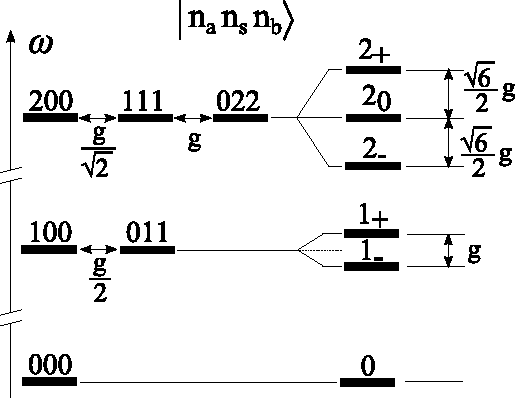
\includegraphics[width=0.6\textwidth]{./figs_Komar2013/fig1b.pdf}
\caption
[Lower level diagram of 2+1 optomechanical system]
{ 
  \label{fig:cartoon_b}
  Level diagram showing  the  relevant  zero-, one- and two-photon states
  at zero temperature and under the three-mode resonance condition
  $\omega_s - \omega_a = \omega_m$. 
  States are labeled by $\ket{n_a n_s n_b}$ denoting
  the number $n_a$ ($n_s$) of antisymmetric
  (symmetric) photons and the number of phonons $n_b$.
   The optomechanical coupling $g$ splits
   the degeneracy of states  $\ket{n_a n_s n_b}$ and
  $\ket{n_a-1, n_s+1, n_b+1}$.}
\end{figure}
The nonlinear terms proportional to $g$ 
in  Eq.~\eqref{eq:Hamiltonian_eff} 
describe 
coherent photon exchange between the two optical modes
mediated by
absorption or emission of a phonon. 
The resulting low energy level diagram
%populated by  weakly driving  the
%antisymmetric mode 
is shown in
\reffig{fig:cartoon_b},
%for $\omega_m=2J$. 
where $\ket{n_a n_s n_b}$ represents a state with
$n_a$ and $n_s$
photons in the $c_a$ and $c_s$ modes, and $n_b$ phonons 
in the mechanical mode.
%and with states labelled  by $\ket{n_a n_s n_b}$.
In the absence of a drive we
diagonalize $H$  in this
few-photon subspace, yielding
the eigenstates %shown in \reffig{fig:cartoon}(b)),
\bal
	\label{eq:ket0}\ket{0} &=& \ket{000},
	\\
	\label{eq:ket1pm}\ket{1_\pm} &=& \frac{1}{\sqrt{2}}\left(\ket{100} \pm
	\ket{011}\right),
	\\
	\label{eq:ket2pm}\ket{2_\pm} &=& \frac{1}{\sqrt{6}}\left(\ket{200}\pm
	\sqrt{3}\ket{111} + \sqrt{2}\ket{022}\right), 
	\\
	\label{eq:ket20}\ket{2_0} &=& \frac{1}{\sqrt{3}}\left(\sqrt{2}\ket{200} -
	\ket{022}\right).
\eal
Note that in the diagonal basis the weak driving field couples 
all states with photon number differing by one. 
In the following sections we use this low energy Hilbert space
to understand photon correlations in the system.






In addition to the coherent evolution modeled  by the
Hamiltonian $H$, we describe optical and mechanical dissipation
using a master equation for the system density
operator $\rho$,
\bal
\label{eq:master_equation}
%	\frac{d}{dt}
	\dot \rho &=& -i[H,\rho] + \kappa \DD[c_a]\rho +
	\kappa \DD[c_s]\rho \\
	&& \qquad + \frac{\gamma}{2}(N_{\text{th}}+1) \DD[b]\rho +
	\frac{\gamma}{2}N_{\text{th}}\DD[b\+]\rho,
\eal
where $H$ is  given by \refeq{eq:Hamiltonian_eff}, $2\kappa$ and $\gamma$ are
energy decay rates for the optical and mechanical modes, respectively,
$N_{\text{th}}$ is the thermal phonon population and  $\DD[\hat o] \rho =
2\hat o \rho \hat o\+ - \hat o\+ \hat o \rho - \rho \hat o\+ o$.
Below we study nonlinear effects at the level
of single photons, both numerically and analytically,
by solving \refeq{eq:master_equation}
approximately in the limit of weak
optical driving, $\Omega \equiv \Omega_a\ll
\kappa$.


%%%%%%%%%%%%%%%%%%%%%%%%%%%%%%%%%%%%%%%%
%%%%%%%%%%%%%%%%%%%%%%%%%%%%%%%%%%%%%%%%
\section{Equal-time correlations}
\label{sect:Averages}

 
\subsection{Average transmission and reflection}


Before focussing on photon-photon correlations, we first
study
the average transmission through the cavity, which is proportional
to the mean intracavity photon number. In
\reffig{fig:spectrum_a} and \ref{fig:spectrum_b} we show the 
intracavity photon number of the
two optical modes,
\bel
	\label{eq:nAvg}
	\bar n_i = \ev{c_i\+ c_i},
\eel
where $i =a,s$, and angle brackets denote the steady state average.
At $\Delta/g =
\pm \frac{1}{2}$, both transmission curves exhibit a maximum,
indicating that the driving field is in resonance 
with an eigenmode of the system.
The position of these peaks can be  understood from the level diagram shown
in Fig.~\ref{fig:cartoon_b}, which at finite $g$ shows a splitting
of the lowest photonic states into a doublet, $|1_\pm\rangle=(|100\rangle
\pm|011\rangle)/\sqrt{2}$.
% ==================================
% \begin{figure}[tb]
% \centering
%   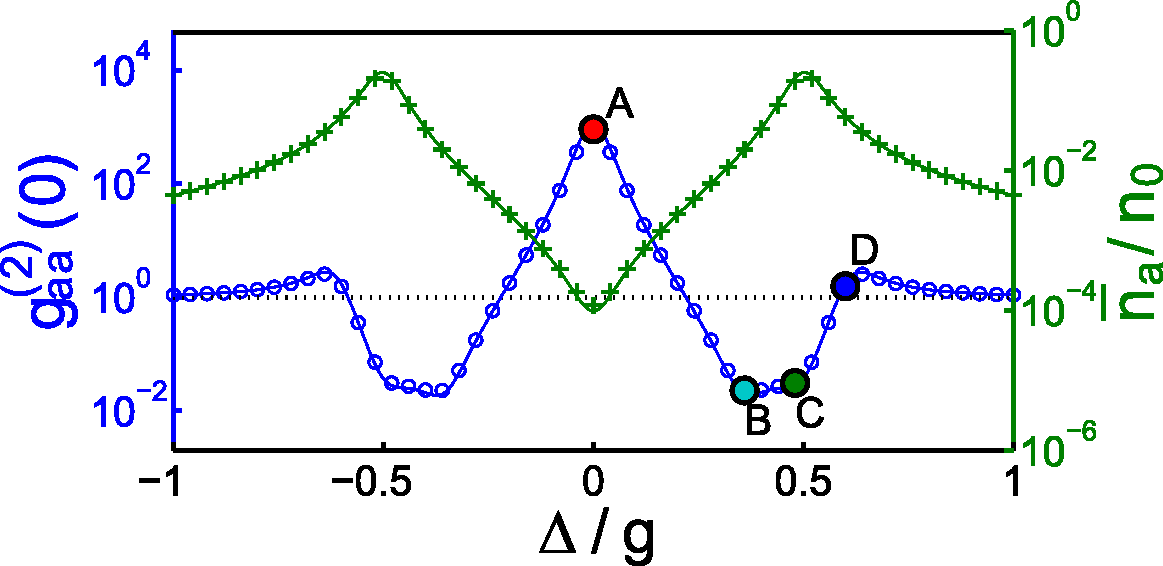
\includegraphics[width=0.45\textwidth]{./figs_Komar2013/fig2a.pdf}\quad
%   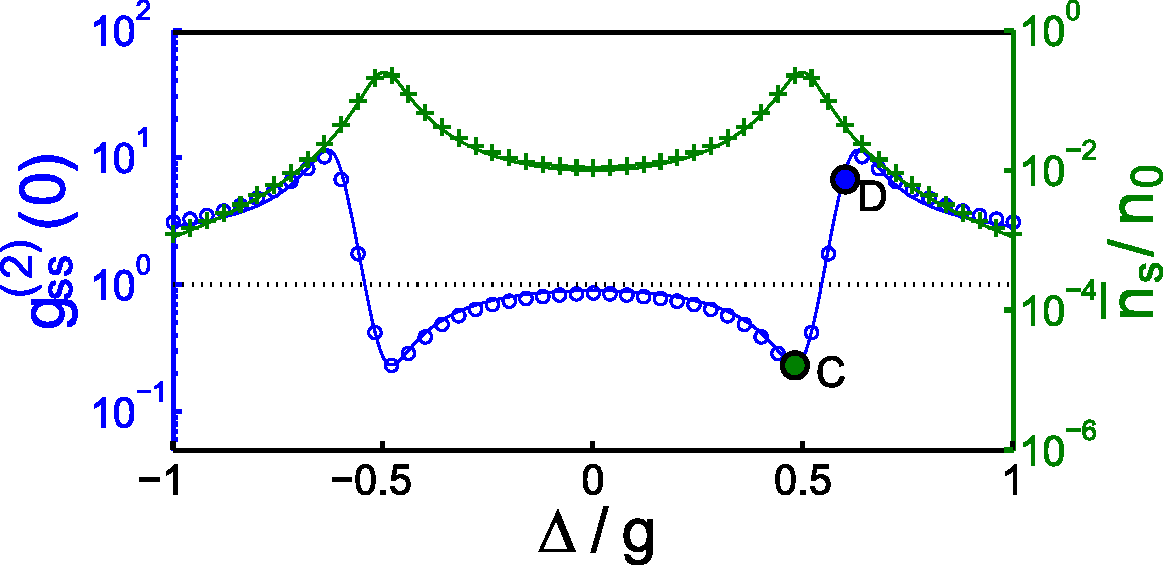
\includegraphics[width=0.45\textwidth]{./figs_Komar2013/fig2b.pdf}\\
%   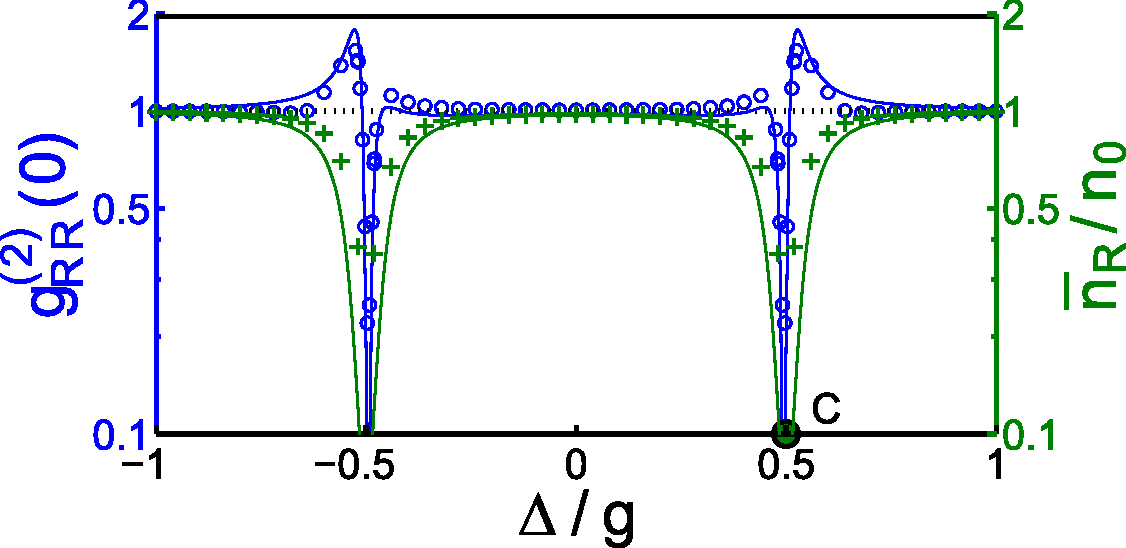
\includegraphics[width=0.45\textwidth]{./figs_Komar2013/fig2c.pdf}\quad
%   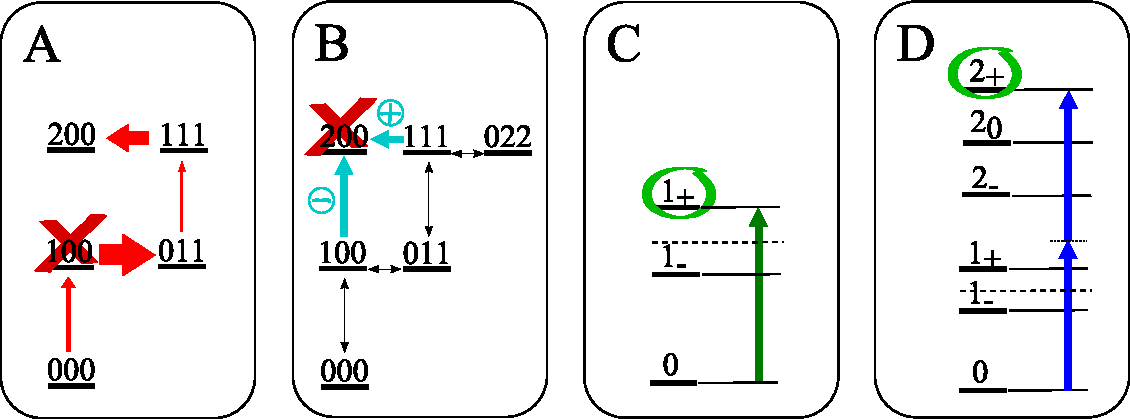
\includegraphics[width=0.45\textwidth]{./figs_Komar2013/fig2d.pdf}
%   \caption{
%   \label{fig:spectrum}(Color online)
%   (a) Normalized average photon number (green ``$+$")
%   and photon-photon correlation function (blue ``$\circ$")
%   for driven mode $c_a$
%   as a function of laser detuning at zero temperature.
%   Solid lines are calculated from analytic model
%   (see Eqs.~(\ref{eq:na}-\ref{eq:g2AA}))
%   and points show full numerical calculation.
%   The average photon number is
%   normalized by $n_0 = (\Omega/\kappa)^2$.
%   (b) Same as in (a) for the undriven mode $c_s$,
%   and
%   (c) for the reflected field $c_R$.
%   In all plots we took
%    $g/\kappa = 20$ and $\gamma/\kappa$ = 0.2.
%   Dots mark features seen at values of
%   detuning $\Delta/g = 0 \text{ (A)}, \frac{1}{\sqrt{8}} \text{ (B)},
%   \frac{1}{2} \text{ (C)}$ and  $\frac{\sqrt{6}}{4} \text{ (D)}$. 
%   The
%   small discrepancy between the analytic and numerical results
%   in (c) is due to the approximation
%   $g/\kappa \gg 1$   to  
%   simplify the expressions in Eqs.~(\ref{eq:na}-\ref{eq:g2AA}).
%   Bottom panels A-D illustrate the origin of these features as explained in the text.
%   Suppression  (enhancement) of the
%   steady state population of a specific level is
%   indicated by a red X (green circle).
%   }
% \end{figure}
% ==================================

\begin{figure}
\centering
  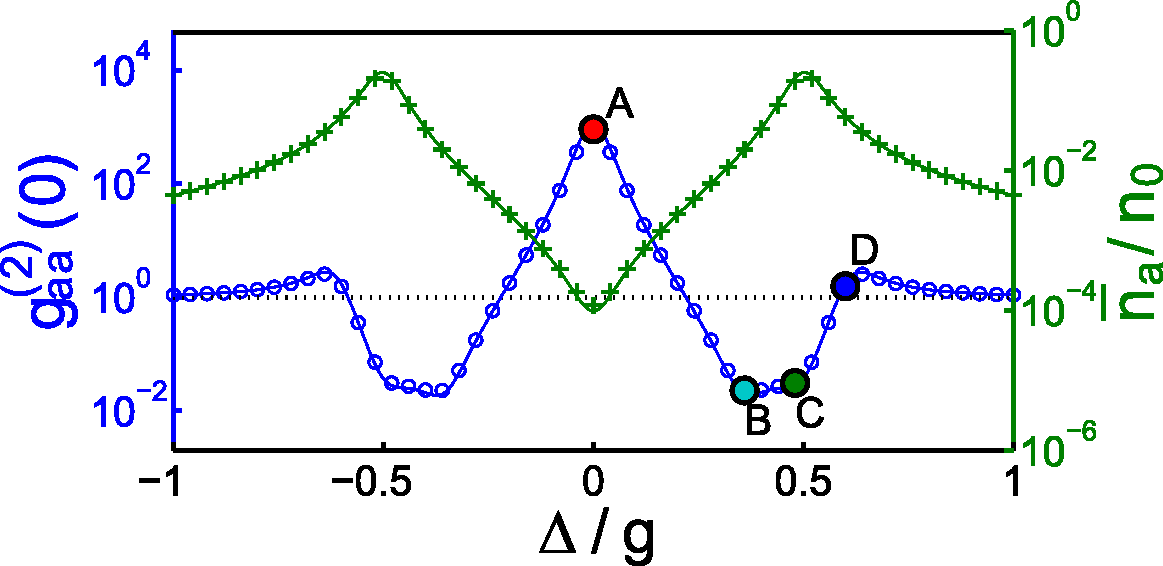
\includegraphics[width=0.8\textwidth]{./figs_Komar2013/fig2a.pdf}
  
  \caption
  [Photon statistics in mode anti-symmetric mode, $a$]
  {
  \label{fig:spectrum_a}
  Normalized average photon number (green ``$+$")
  and photon-photon correlation function (blue ``$\circ$")
  for driven mode $c_a$
  as a function of laser detuning at zero temperature.
  Solid lines are calculated from analytic model
  (see Eqs.~(\ref{eq:na}-\ref{eq:g2AA}))
  and points show full numerical calculation.
  The average photon number is
  normalized by $n_0 = (\Omega/\kappa)^2$. ($g/\kappa = 20$ and $\gamma/\kappa$
  = 0.2)
  }
\end{figure}

\begin{figure}
\centering
  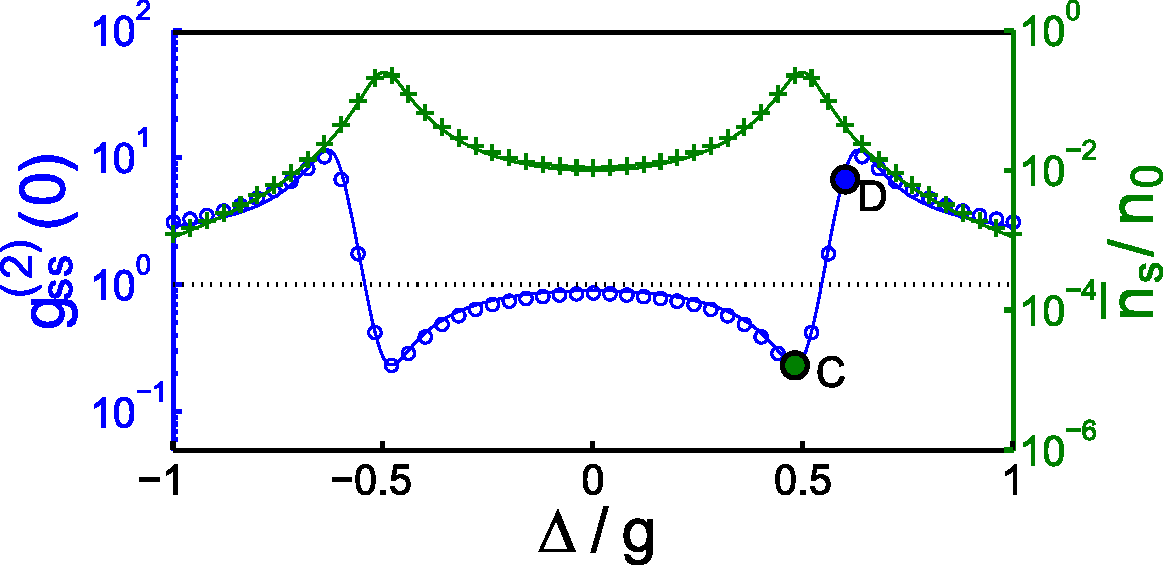
\includegraphics[width=0.8\textwidth]{./figs_Komar2013/fig2b.pdf}
  \caption
  [Photon statisics in mode symmetric mode, $s$]
  {
  \label{fig:spectrum_b}
  Normalized average photon number (green ``$+$")
  and photon-photon correlation function (blue ``$\circ$")
  for the undriven mode $c_s$
  as a function of laser detuning at zero temperature.
  Solid lines are calculated from analytic model
  (see Eqs.~(\ref{eq:na}-\ref{eq:g2AA}))
  and points show full numerical calculation.
  The average photon number is
  normalized by $n_0 = (\Omega/\kappa)^2$. ($g/\kappa = 20$ and $\gamma/\kappa$
  = 0.2)
  }
\end{figure}
 
\begin{figure}
\centering
  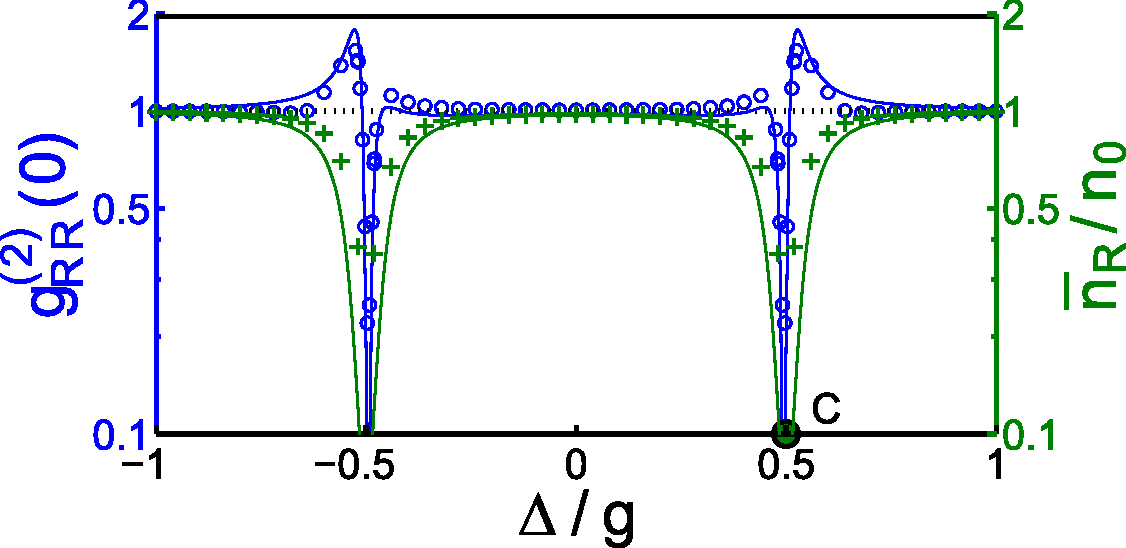
\includegraphics[width=0.8\textwidth]{./figs_Komar2013/fig2c.pdf}
  \caption
  [Photon statistics in the reflected mode, $R$]
  {
  \label{fig:spectrum_c}
  Normalized average photon number (green ``$+$")
  and photon-photon correlation function (blue ``$\circ$")
  for the reflected field $c_R$,
  as a function of laser detuning at zero temperature.
  Solid lines are calculated from analytic model
  (see Eqs.~(\ref{eq:na}-\ref{eq:g2AA}))
  and points show full numerical calculation.
  The average photon number is
  normalized by $n_0 = (\Omega/\kappa)^2$.
  The
  small discrepancy between the analytic and numerical results is due to the
  approximation $g/\kappa \gg 1$   to  
  simplify the expressions in Eqs.~(\ref{eq:na}-\ref{eq:g2AA})
  ($g/\kappa = 20$ and $\gamma/\kappa$ = 0.2)
  }
\end{figure}
 


In addition to the transmission,
we plot the mean reflected photon number
in  \reffig{fig:spectrum_c}.
As discussed below, the reflected 
photon statistics
can also exhibit signatures of
nonlinearity.
We  calculate properties of the reflected light
using the
annihilation operator 
$c_R = c_a + i\frac{\Omega}{\kappa}$, obtained from standard input-output relations
for a symmetric two-sided cavity (see Appendix
\ref{App: Reflection}).
%$c_R = c_a + i\frac{\Omega}{\kappa}$.
The mean reflected photon number
$\bar n_R = \ev{c_R\+ c_R}$
is plotted in \reffig{fig:spectrum_c}.
%shows the reflected photon number, 
%$\bar n_R = \ev{c_R\+ c_R}$. 
At $\Delta/g = \pm \frac{1}{2}$, 
the average reflection has a minimum where the
average transmission has a maximum. 
Note that in contrast to a single cavity, 
even on resonance the transmission probability
is less than unity and the reflection probability
remains finite.



\subsection{Intensity correlations}
\label{sec:onetime_correlation}

To  characterize nonclassical 
photon statistics in the light transmitted though the OMS
we study the equal-time photon-photon correlation
functions,
\bel
	\label{eq:g2(0)}
	g^{(2)}_{ii}(0)
	= \frac{\ev{c_i\+ c_i\+
	c_i  c_i }}{\ev{c_i\+ c_i}^2} ,
\eel
where all operators are evaluated at the same time and $i = a,s, R$. 
A normalized correlation of
$g^{(2)}_{ii}(0)< 1$ indicates photon anti-bunching, and the limit
$g^{(2)}_{ii}(0)\rightarrow 0$ corresponds to the 
complete photon blockade regime
in which two photons never occupy the cavity
at the same time.
The solid curves show $g^{(2)}_{aa}(0)$ in \reffig{fig:spectrum_a},
$g^{(2)}_{ss}(0)$ in \reffig{fig:spectrum_b} and $g^{(2)}_{RR}(0)$ 
\reffig{fig:spectrum_c} as a function of the laser  detuning and in the limit of
weak driving $\Omega/\kappa \ll1 $.
%for modes $c_a$, $c_s$ and the reflected
%mode $c_R$, respectively.
The most pronounced features of these correlation functions occur at 
$|\Delta|/g = 0, \frac{1}{\sqrt{8}}, \frac{1}{2} \text{ and }\frac{\sqrt{6}}{4}$, 
as marked by
dots A, B, C and D, respectively. 
As we explain in detail in the following analysis, 
%Fig.~\ref{fig:spectrum}, 
we find that the photon bunching at A and
anti-bunching at B are the result of destructive 
quantum interference, while the 
features at points C and D arise from 
one- and two-photon resonances. 

%As illustrated in the bottom panel of
%Fig.~\ref{fig:spectrum}, 
%the photon bunching at A and
%anti-bunching at B arise from the suppression 
%of populations in states
%$|100\rangle$ and $|200\rangle$ respectively,
%due to destructive quantum interference
%(depicted by a red X).
%In contrast, the features at points C and D arise from 
%one- and two-photon
%resonances of the coupled system (indicated by a green O).
%These features can be understood
%in terms of a simple analytic model as we now discuss.

To gain insight into the two photon correlation functions shown in 
%We can capture the 
%features in  
\reffig{fig:spectrum_a}, \ref{fig:spectrum_b} and \ref{fig:spectrum_c},
we develop  an approximate analytic model 
for the system 
by considering only the
six levels shown in \reffig{fig:cartoon_b}.
Assuming that the system is initially prepared in $|000\rangle$, these are
the only levels significantly populated by weakly driving the
$c_a$ mode. We make the ansatz \cite{Carmichael1991}
\bel
\label{eq:psi}
\begin{split}
	\ket{\psi} =&\quad A_{000}\ket{000} + A_{100}\ket{100} + A_{011}\ket{011}\\
	&+ A_{200} \ket{200} + A_{111} \ket{111} + A_{022} \ket{022},
\end{split}
\eel
and describe the dynamics by evolving $|\psi\rangle$ under the action of the
non-Hermitian Hamiltonian, $\tilde{H} = H -i\left[\kappa c_a\+ c_a + \kappa
c_s\+ c_s + \frac{\gamma}{2} b\+ b\right]$. 
This approach allows us to evaluate
intensities up to order $\Omega^2$ and two-point correlation up to order
$\Omega^4$, since the neglected quantum jumps
lead to higher order corrections.
By neglecting the typically small mechanical decay rate
$\gamma \ll \kappa$,
the amplitudes in \refeq{eq:psi} then satisfy
\bal
	\label{eq:c000}\dot A_{000} &=& 0,\\[0.2cm]
	\dot A_{100} &=& -i\frac{g}{2} A_{011} -i\Omega A_{000} -
	\tilde\kappa A_{100},\\
	\label{eq:c011}
	\dot A_{011} &=& -i\frac{g}{2} A_{100} - \tilde\kappa A_{011},\\[0.2cm]
	\dot A_{200} &=& -i\frac{g}{\sqrt{2}} A_{111} -i\sqrt{2}\Omega A_{100}
	-2\tilde\kappa A_{200},\\
	\dot A_{111} &=& -i\frac{g}{\sqrt{2}} A_{200} -ig A_{022} - i\Omega A_{011} -
	2\tilde\kappa A_{111},\\
	\label{eq:c022}
	\dot A_{022} &=& -ig A_{111} -2\tilde\kappa A_{022},
\eal
where $\tilde \kappa = \kappa -i\Delta$. 
It is straightforward to solve
Eqs. (\ref{eq:c000}--\ref{eq:c022}) for the steady state amplitudes 
(see Appendix \ref{sect:App:steady_state}).
%\ref{sect:App:steady_state}
To lowest order in $\Omega/\kappa$  the mean
occupation numbers are $\bar n_a=|\bar A_{100}|^2$, $\bar n_s=|\bar A_{011}|^2$
and $\bar n_R=|\bar A_{100}+i\Omega/\kappa|^2$, where $\bar A$ denote
steady state amplitudes. We obtain
\bal
	\label{eq:na}
	\frac{\bar n_a}{n_0} &=&
		\frac{
			\kappa^2\left[R_\kappa(0)\right]^{1/2}
		}
		{
			R_\kappa\left(\frac{g}{2}\right)
		},\\
	\frac{\bar n_s}{n_0} &=&
		\frac{
			g^2\kappa^2
		}
		{
			4R_\kappa\left(\frac{g}{2}\right)
		},\\
	\frac{\bar n_R}{n_0} &\approx &
		\frac{
			\left[R_{\kappa/2}\left(\frac{g}{2}\right)\right]^2
		}
		{
			\left[R_\kappa\left(\frac{g}{2}\right)\right]^2
		},
\eal
where 
$R_K(\omega) = \left[K^2 +
(\Delta-\omega)^2\right]\left[K^2 + (\Delta+\omega)^2\right]$
and
$n_0 = (\Omega/\kappa)^2$.
%and $R_K(\omega) = \left[K^2 +
%(\Delta-\omega)^2\right]\left[K^2 + (\Delta+\omega)^2\right]$. 
From the 
factors $R_K(\omega)$ in the denominators  (numerators)
in these expressions, we obtain the positions
of the resonances  (antiresonances) in the 
average intracavity photon numbers, in excellent
agreement with the numerical results
shown in \reffig{fig:spectrum_a}, \ref{fig:spectrum_b} and
\ref{fig:spectrum_c}.
%We discuss these features in  detail below.
Our six-level model also provides the
equal-time correlations
(see Appendix \ref{sect:App:steady_state}),
%for
%which we find (see Appendix)
%\ref{sect:App:steady_state})
\bal
	g^{(2)}_{aa}(0) &=&
		\frac{
			R_\kappa\left(\frac{g}{\sqrt{8}}\right)
			R_\kappa\left(\frac{g}{2}\right)
		}
		{
			R_\kappa(0)
			R_\kappa\left(\frac{\sqrt{6}}{4}g\right)
		},
		\label{eq:g2aa}
		\\
	g^{(2)}_{ss}(0) &=&
		\frac{ 2
			R_\kappa\left(\frac{g}{2}\right)
		}
		{
			R_\kappa\left(\frac{\sqrt{6}}{4}g\right)
		},\\
	g^{(2)}_{RR}(0) &\approx &
		\frac{
			R_\kappa\left(\frac{g}{2}\right)
			R_{16\kappa^3/g^2}\left(\frac{g}{2}-\frac{2\kappa^2}{g}\right)
		}
		{
			\left[R_{\kappa/2}\left(\frac{g}{2}\right)\right]^2
		}.
		\label{eq:g2AA}
\eal
Again, these expressions are in agreement with
the features seen in the numerical results in \reffig{fig:spectrum_a},
\ref{fig:spectrum_b} and \ref{fig:spectrum_c}.
The positions of maxima and minima are
seen directly by the arguments of
the factors $R_K(\omega)$. 
Note that we assumed $g/\kappa \gg 1$ to
obtain the simplified
expressions in Eqs.~(\ref{eq:g2aa}-\ref{eq:g2AA}),
but we retained the 
shift of order $g (\kappa / g)^2$ in
the argument in \refeq{eq:g2AA}
%in the argument of the second $R$ symbol,
because this shift is larger than the width of 
the antiresonance.

%we approximated
%\refeq{eq:g2AA}, 


%To gain further insight on the positions of 
%the features seen in \reffig{fig:spectrum}
%and described by Eqs.~(\ref{eq:na}--\ref{eq:g2AA}), we 
%diagonalize $H$ in \refeq{eq:Hamiltonian_0} in the
%six-level subspace of \refeq{eq:psi}.
%This yields the following eigenstates (see
%\reffig{fig:cartoon}(b)):
%\bal
%	\label{eq:ket 0}\ket{0} &=& \ket{000},
%	\\
%	\label{eq:ket 1pm}\ket{1_\pm} &=& \frac{1}{\sqrt{2}}\left(\ket{100} \pm
%	\ket{011}\right),
%	\\
%	\label{eq:ket 2pm}\ket{2_\pm} &=& \frac{1}{\sqrt{6}}\left(\ket{200}\pm
%	\sqrt{3}\ket{111} + \sqrt{2}\ket{022}\right), 
%	\\
%	\label{eq:ket 2 0}\ket{2_0} &=& \frac{1}{\sqrt{3}}\left(\sqrt{2}\ket{200} -
%	\ket{022}\right).
%\eal
%In the diagonal basis, the weak drive couples all levels with total photon
%number $n$ to all levels with $n\pm 1$ photons.
%Some of the features arise simply from detuning
%the drive through one- or two-photon resonance
%with these eigenstates of the coupled OM system.

\begin{figure}
\centering
  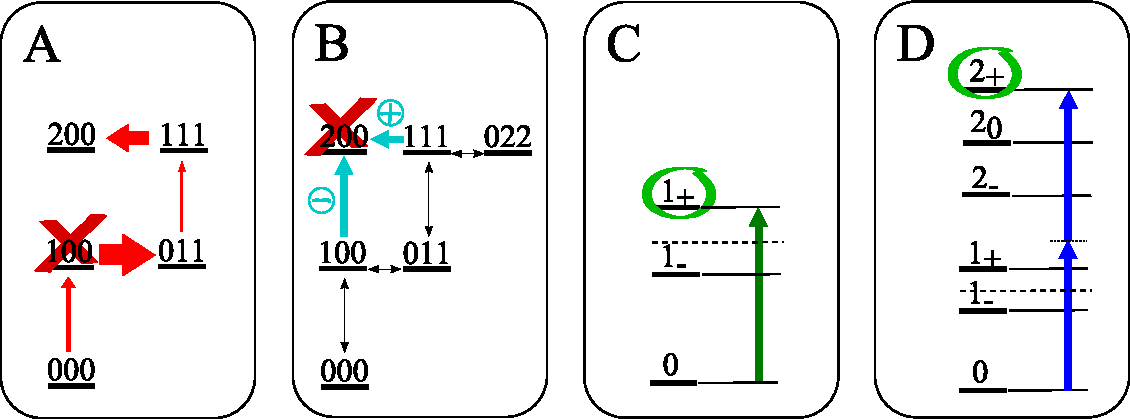
\includegraphics[width=0.9\textwidth]{./figs_Komar2013/fig2d.pdf}
  \caption
  [Illustration of dominant processes]
  {
  \label{fig:spectrum_d}
  Illustration of the origin of the features marked with A,B,C and D on
  \reffig{fig:spectrum_a}, \ref{fig:spectrum_b} and \ref{fig:spectrum_c} as
  explained in the text.
  Suppression  (enhancement) of the
  steady state population of a specific level is
  indicated by a red X (green circle).
  }
\end{figure}
We now discuss each feature
in \reffig{fig:spectrum_a}, \ref{fig:spectrum_b} and \ref{fig:spectrum_c} in
terms of our six-level model together with the diagonal basis
in Eqs.~(\ref{eq:ket0}-\ref{eq:ket20}).
First, at 
detuning $\Delta = 0$ (point A in \reffig{fig:spectrum_a})
we see $g^{(2)}_{aa}(0)>1$, indicating bunching.  
This is due to destructive interference that
suppresses
the population in  $\ket{100}$ 
(panel A in \reffig{fig:spectrum_d}), and
can be understood as the system being
driven into a dark state,
$\ket{d} \propto g \ket{000} - \Omega \ket{011}$, similar to
electromagnetically induced 
transparency (EIT) \cite{Lukin2003, Weis2010}.
In the dark state, $\ket{011}$ remains populated,
% KS: I changed 110 -> 100 here
% SB: both incorrect, should be 011 
%by the weak drive, 
allowing transitions to $\ket{111}$
which in turn is strongly coupled to
$\ket{200}$.
The net result is a relative 
suppression of the probability to have one photon
compared to two photons
in the driven mode, 
leading to bunching at $\Delta = 0$.
Second, at detuning $\Delta = g/\sqrt{8}$ 
(point B), 
mode $c_a$ shows anti-bunching
due to a suppressed two-photon probability.
Again, this is due to destructive interference, or
the presence of a dark state in which
$\ket{200}$ remains unpopulated
(panel B).
Third, at detuning $\Delta = \frac{g}{2}$ 
(point C), 
all  modes show anti-bunching.
This is due to
a one-photon  resonant transition
$\ket{0} \rightarrow \ket{1_+}$ 
(panel C).
Finally, at detuning $\Delta = \frac{\sqrt{6}}{4}g$ 
(point D), 
both $c_a$ and $c_s$ show bunching due
to a two-photon resonant transition
$\ket{0} \rightarrow \ket{2_+}$
(panel D).
% KS: I replaced cartoon -> inset
% SB: inset -> panel



\subsection{Absence of two-photon resonance at $\Delta = 0$}

At first glance,
the level diagram in \reffig{fig:cartoon_b} together with
bunching 
in \reffig{fig:spectrum_a} 
suggest a two-photon resonance
at zero detuning $\Delta = 0$,
where the energy of the
eigenstate $\ket{2_0}$ is equal to the energy of two drive photons.
However, 
as discussed above,
the bunching at $\Delta = 0$ arises 
entirely from
the suppression of a one-photon population;
further, we 
find that the expected two-photon resonance is 
cancelled by  interference.
This can be seen from a second order perturbative 
calculation of the two-photon Rabi frequency $\Omega_{0,2_0}^{(2)}$ for the transition 
$|0\rangle\rightarrow |2_0\rangle$.  
The two-photon state $\ket{2_0}$ can be
populated by the drive 
$H_{\rm dr} = \Omega (c_a^\dag + c_a)$ 
from state $\ket{0}$ 
via two intermediate one-photon
eigenstates, $\ket{1_\pm}$ given by \refeq{eq:ket1pm},
with energies $\omega_{1_\pm} = -\Delta \pm \frac{g}{2}$
in the rotating frame.
The resulting Rabi frequency is
\bel
\label{eq:fgr}
	\Omega_{0,2_0}^{(2)} = \sum_{n=1_-, 1_+}
\frac{\ev{2_0| H_{\rm dr} |n}\ev{n| H_{\rm dr} |0}}{\omega_n},
\eel
which vanishes at $\Delta=0$ 
%the two-photon Rabi frequency vanishes
as a consequence of destructive interference between the two amplitudes. 
The exact cancellation is lifted
by including finite dissipation and the full spectrum;
%leading to finite population in $\ket{2_0}$;
nonetheless this simple argument shows that
the expected two-photon resonance at $\Delta = 0$
is strongly 
suppressed.


%$\kappa$ or $\gamma$ the exact cancellation is lifted, 
%and
%the resulting small, but finite population in $|2_0\rangle$ is responsible for
%the antibunching in point A.


%This can be seen from a second order 
%Fermi's golden rule calculation.
%The two-photon state $\ket{2_0}$ can be
%populated by the driving field from state $\ket{0}$ 
%via  two intermediate one-photon
%eigenstates, $\ket{1_+}$ and $\ket{1_-}$. 
%The total transition rate is
%$\Gamma_{\ket{0}\rightarrow \ket{2_0}} = 2\pi \left| M \right|^2
%\delta\left(\omega_0 - \omega_{2_0} \right)$,
%where in the rotating frame
%$\omega_0 = \omega_{2_0} = 0$, $\omega_{1_\pm} = -\Delta \pm \frac{g}{2}$,
%and 
%\bel
%\label{eq:fgr}
%	M = \sum_{n=1_-, 1_+}
%\frac{\ev{2_0| H_{\rm dr} |n}\ev{n| H_{\rm dr} |0}}{\omega_n} = 0.
%\eel
%We see that on resonance,
%$\Delta = 0$, the total rate vanishes
%%$\Gamma_{\ket{0}\rightarrow \ket{2_0}}=0$.
%%This is a consequence of 
%due to
%destructive interference of
%the two-photon
%amplitudes that would allow the transition.
%\sdb{Fix this.}
%Of course, for non-zero $\kappa$ or $\gamma$ this exact interference is lifted, and the resulting small, but finite population in $|2_0\rangle$ is responsible for the antibunching in point A.  



%This can be seen from a second order perturbative calculation of the two photon Rabi frequency $\Omega_{0,2_0}^{(2)}$ for the transition 
%$|0\rangle\rightarrow |2_0\rangle$.  The two-photon state $\ket{2_0}$ can be
%populated by the driving field from state $\ket{0}$ 
%via  two intermediate one-photon
%eigenstates, $\ket{1_+}$ and $\ket{1_-}$, which in the rotating frame
%have energies $\omega_{1_\pm} = -\Delta \pm \frac{g}{2}$, respectively. 
%Therefore, 
%\bel
%\label{eq:fgr}
%	\Omega_{0,2_0}^{(2)} = \sum_{n=1_-, 1_+}
%\frac{\ev{2_0| H_{\rm dr} |n}\ev{n| H_{\rm dr} |0}}{\omega_n},
%\eel
%and we see that on resonance $\Delta=0$ the two-photon Rabi-frequency vanishes as a consequence of destructive interference between the two amplitudes. Of course, for non-zero $\kappa$ or $\gamma$ this exact interference is lifted, and the resulting small, but finite population in $|2_0\rangle$ is responsible for the antibunching in point A.  



Further evidence of the absence of a
two-photon resonance at $\Delta=0$ is
the lack of bunching in the undriven mode in  
\reffig{fig:spectrum_b}.
If there were a two-photon resonance,
one would expect that bunching
should also occur in the undriven mode,
since the state $\ket{2_0}$ involves both $c_a$
and $c_s$ modes. 
This is indeed the case
at detuning $\Delta = \frac{\sqrt{6}}{4} g$
(see point D in \reffig{fig:spectrum_b}),
where
both modes show bunching as a result of
two-photon resonance.
In contrast, we see  no bunching in
the undriven mode at $\Delta = 0$. 
%due to the
%cancellation of two-photon resonance by interference.
This supports our conclusion that the observed
bunching at $\Delta=0$ arises 
from suppression of 
population in $\ket{100}$ due to interference,
as discussed in Section \ref{sec:onetime_correlation},
and not from two-photon resonance.
%Instead, this bunching arises
%from a suppression of the one-photon amplitude
%$A_{100}$
%as discussed in Section \ref{sec:onetime_correlation}.
As discussed above, this interference
does not suppress population in 
$\ket{011}$,
so we do not expect
bunching in the $c_s$ mode from this effect.
% ==================================
\begin{figure} 
\centering
  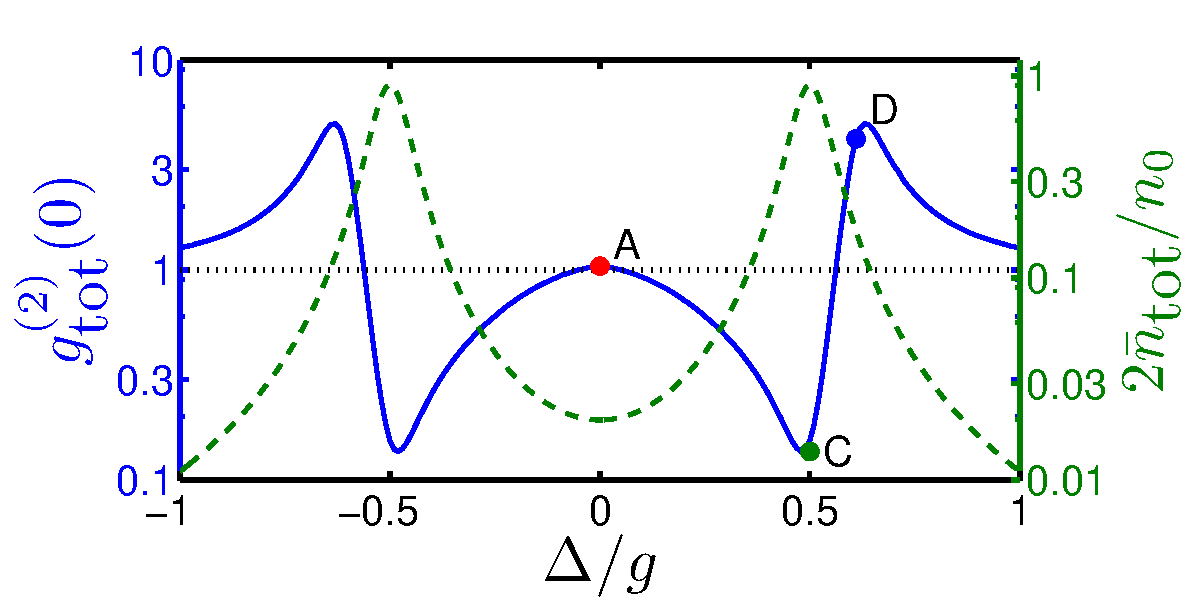
\includegraphics[width=0.8\textwidth]{./figs_Komar2013/fig3.pdf}
  \caption
  [Aggregate photon statistics of both modes]
  {
  \label{fig:populations}
  Average number (green dashed) and intensity correlation
  (blue solid)
  of total photon number in the coupled OM system.
  Parameters are the same as in \reffig{fig:spectrum_a},
  and dots mark the same detunings.
  One- and two-photon resonances are
  seen at C and D,
  but we see no bunching in the
  total photon number at 
  $\Delta = 0$ (point A).
%  is where a two-photon transition
%  $\ket{0}\rightarrow\ket{2_0}$ is naively expected.
  This reflects the lack
  of two-photon resonance due to 
  destructive interference (see \refeq{eq:fgr}).  } 
\end{figure}
% ==================================

Finally, to confirm our intuitive picture we plot the
intensity correlation function, 
$g^{(2)}_{\text{tot}}(0) =
\ev{n_{\text{tot}}(n_{\text{tot}}-1)}/\ev{n_{\text{tot}}}^2$,
of the total photon number, $n_{\text{tot}} = n_a +
n_s$,
in the coupled OM system in
\reffig{fig:populations}. 
The probability to find one photon in the combined
cavity is maximal at $\Delta/g=\pm \frac{1}{2}$ 
due to one-photon resonance.
Similarly, we  
observe antibunching at point C
and bunching at point D,
due  to interference and two-photon resonance
respectively,
as discussed 
in Section \ref{sec:onetime_correlation}.
%The two-photon probability also has a peak at $\Delta/g=\pm \frac{1}{2}$, since
%a second photon can enter the cavity off-resonantly.
%In addition, the two-photon probability has peaks at 
%$\Delta / g  = \pm \sqrt{6} /4$ due to two-photon resonances.  
However, we find neither bunching nor antibunching
at $\Delta = 0$, 
demonstrating the absence of a two-photon resonance
despite the fact that $\ket{2_0}$ lies at twice the
drive frequency.



%Finally, to confirm our intuitive picture we plot the
%total photon number and $g^{(2)}(0)$ in steady state in
%\reffig{fig:populations}.
%The number of photons ($n_\text{tot} = n_a + n_s$) in the combined
%cavity is maximal and $g^{(2)}_\text{tot}(0) =
%\ev{n_\text{tot}(n_\text{tot}-1)}/\ev{n_\text{tot}}^2$
%is minimal at $\Delta/g=\pm \frac{1}{2}$ due to one-photon resonance causing anti-bunching.
%The $g^{(2)}_\text{tot}(0)$ has peaks at 
%$\Delta / g  = \pm \sqrt{6} /4$ due to two-photon resonances.  
%However, there
%is no peak ($g^{(2)}_\text{tot}(0) \approx 1$) at $\Delta = 0$, 
%demonstrating the absence of a two-photon resonance
%despite the fact that $\ket{2_0}$ lies at the twice the
%drive frequency.

 


\subsection{Finite temperature}

\begin{figure}
\centering
  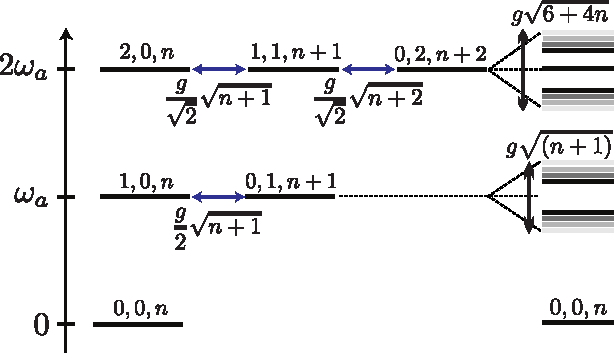
\includegraphics[width=0.8\textwidth]{./figs_Komar2013/fig4a.pdf}
  \caption
  [Temperature dependence of the relevant levels]
  {
  \label{fig:thermal_g2_a}
  Level diagram showing the
  six states populated by the drive from level $|0,0,n\rangle$ (left), 
  and the associated
  eigenmodes (right) with $n$-dependent splittings.
}
\end{figure} 

\begin{figure}
\centering
  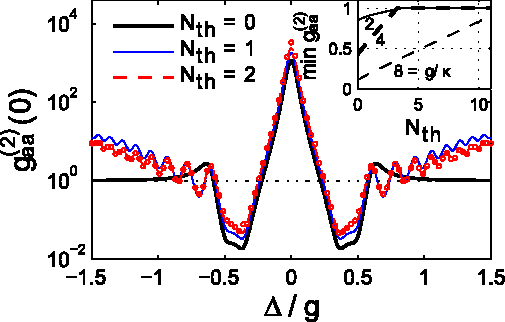
\includegraphics[width=0.8\textwidth]{./figs_Komar2013/fig4b.pdf}
  \caption
  [Effect of non-zero temperature on photon statistics of mode $a$]
  {
  \label{fig:thermal_g2_b}
  Driven mode correlation function $g^{(2)}_{aa}(0)$
  for thermal mechanical occupation $N_{\rm th} = 0,1,2$.
  Solid lines show the analytic calculation with $\gamma \rightarrow 0$,
   and  dots show the full numerical results for $N_{\rm th} = 2$ only.
  The inset shows the minimal $g^{(2)}_{aa}(0)$ as a function of $N_{\rm th}$ 
  for several
  coupling strengths. 
  Parameters are $g/\kappa=20$, and (for numerics) $\gamma/\kappa =  10^{-3}$.
}
\end{figure} 

\begin{figure}
\centering
  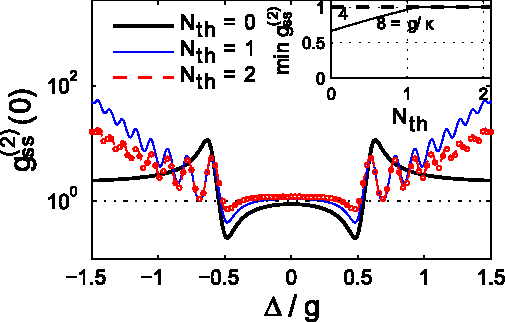
\includegraphics[width=0.8\textwidth]{./figs_Komar2013/fig4c.pdf}
  \caption
  [Effect of non-zero temperature on photon statistics of mode $s$]
  {
  \label{fig:thermal_g2_c}
  Undriven mode correlation function $g^{(2)}_{ss}(0)$
  for thermal mechanical occupation $N_{\rm th} = 0,1,2$.
  Solid lines show the analytic calculation with $\gamma \rightarrow 0$,
   and  dots show the full numerical results for $N_{\rm th} = 2$ only.
  The inset shows the minimal $g^{(2)}_{ss}(0)$ as a function of $N_{\rm th}$ 
  for several
  coupling strengths. 
  Parameters are $g/\kappa=20$, and (for numerics) $\gamma/\kappa =  10^{-3}$.
}
\end{figure} 


So far in our analysis
we have focused on the case where the mechanical
system is prepared in its vibrational 
ground state, $|0_m\rangle$. 
This
condition can be achieved using high frequency resonators 
operated at cryogenic
temperatures \cite{O'Connell2010}, 
and in the limit of weak driving $\Omega/\kappa\ll1$ such
that optical
heating of the mechanical mode can be neglected. 
The mechanical groundstate  could also be 
prepared using OM cooling \cite{Metzger2004, Gigan2006, 
Arcizet2006, Kleckner2006, Corbitt2007, 
Schliesser2008,Thompson2008,Wilson2009,
O'Connell2010,Teufel2011,Chan2011},
using an optical mode far-detuned
from the ones we consider  here for 
nonlinear interactions
\cite{Stannigel2012}.
Nonetheless,
in the
following we extend our analytic treatment to the case of finite temperature, 
and show that many of the
nonclassical features are robust even
in the presence of small
but finite thermal occupation of the mechanical mode.


To generalize our previous results we now consider
a finite equilibrium occupation number $N_{\rm th} >0$ of 
the mechanical mode,
but still assume that $\gamma(N_{\rm th}+1) \ll\kappa,g$. 
Within this approximation we proceed
as above, and
make a similar six-level ansatz as in Eq.~\eqref{eq:psi}
for each phonon number $n$,
%\bel
%\label{eq:psi_thermal}
%\begin{split}
%	&\ket{\psi_n} =\\
%	&\quad A_{0,0,n}\ket{0,0,n} + A_{1,0,n}\ket{1,0,n} +
%	A_{0,1,n+1}\ket{0,1,n+1}\\
%	&+ A_{2,0,n} \ket{2,0,n} + A_{1,1,n+1} \ket{1,1,n+1} \\
%	&+ A_{0,2,n+2}\ket{0,2,n+2},
%\end{split}
%\eel
\bel
\label{eq:psi_thermal}
\begin{split}
	\ket{\psi_n} &=
	 A_{0,0,n}\ket{0,0,n} + A_{1,0,n}\ket{1,0,n} \\
	&+ A_{0,1,n+1}\ket{0,1,n+1} + A_{2,0,n} \ket{2,0,n} \\
	&+ A_{1,1,n+1} \ket{1,1,n+1} 
	+ A_{0,2,n+2}\ket{0,2,n+2},
\end{split}
\eel
 where $\ket{\psi_n}$ includes states up
 to two photons that are connected 
 by the weak drive and coupling $g$,
 starting from the state $|0 0 n\rangle$. 
 As
 shown in Fig.~\ref{fig:thermal_g2_a} the coupling between the states
 within each six-level subspace
 depends explicitly on the phonon number $n$. 
Following the same approach as above,
the amplitudes in Eq.~\eqref{eq:psi_thermal} evolve according to
\bal
       \dot A_{0,0,n} &=& 0,\\
\dot A_{1,0,n} &=& -i \frac{g}{2} \sqrt{n+1} A_{0,1, n+1} -i\Omega A_{,00,n}
-\tilde\kappa A_{1,0,n},\\
\dot A_{0,1,n+1} &=& -i\frac{g}{2} \sqrt{n+1} A_{1,0,n} - \tilde\kappa
A_{0,1,n+1},\\
\dot A_{2,0,0} &=& -i g\sqrt{\frac{n+1}{2}} A_{1,1,n+1} -i\sqrt{2}\Omega
A_{1,0,n}
-2 \tilde\kappa A_{2,0,n},\\
\dot A_{1,1,n+1} &=& -ig\sqrt{\frac{n+1}{2}}  A_{2,0,n} -i
g\sqrt{\frac{n+2}{2}}A_{0,2,n+2} - i\Omega A_{0,1,n+1} - 2\tilde\kappa
A_{1,1,n+1},\qquad \\
\dot A_{0,2,n+2} &=& -ig\sqrt{\frac{n+2}{2}} A_{1,1,n+1} -2\tilde\kappa
A_{0,2,n+2}.
\eal
We solve for the steady state amplitudes within each 
subspace  $n$ and average
the result over the initial thermal phonon distribution,
assuming no coupling between subspaces due to
the small phonon relaxation rate.
We obtain the
average photon numbers
\begin{align}
	\bar n_a=\sum_n \zeta_n |\bar A_{1,0,n}|^2,
	\qquad
	\bar n_s=\sum_n \zeta_n |\bar A_{0,1,n+1}|^2,
\end{align}
where $\zeta_n=e^{-\beta \hbar\omega_m n}(1-e^{-\beta \hbar\omega_m })$ and
$\beta^{-1}=k_B T$.
Similarly, the $g^{(2)}_{ii}(0)$ functions are given by 
\begin{align}
	g^{(2)}_{aa}(0)=&2\sum_n\zeta_n |\bar A_{2,0,n}|^2 / \bar n_a^2,\\
	g^{(2)}_{ss}(0)=&2\sum_n\zeta_n |\bar A_{0,2,n+2}|^2 / \bar n_s^2.
\end{align} 
We provide the expressions for the steady state amplitudes
$\bar A_{2,0,n}$ and $\bar A_{0,2,n+2}$ in the
 Appendix \ref{sect:App:steady_state}.

 





We plot the correlation functions,
$g^{(2)}_{aa}(0)$ in \reffig{fig:thermal_g2_b} and $g^{(2)}_{ss}(0)$ in
\reffig{fig:thermal_g2_c} for different thermal phonon numbers, $N_{\rm th}$. 
Solid lines were calculated from the above
analytic approach with $\gamma \rightarrow 0$, 
and we find excellent agreement with
the full numerical results including small but finite
$\gamma$ (dots, shown only for
thermal occupation $N_{\rm th} = 2$).
We see that the zero temperature
features such as antibunching
survive at finite temperature for sufficiently strong coupling~\cite{Stannigel2012}.
In the insets we plot the minimum antibunching
as a function of thermal occupation number for
several ratios $g / \kappa$. 
Antibunching remains visible up
to a critical thermal phonon number, 
set by $g/\kappa$, 
beyond which the contributions from 
different phonon numbers smear out the effect
and antibunching vanishes.
%\pk{This antibunching vanishes for $N_\text{th}
%\sim g^2/\kappa^2$, which we can understand from estimating $\bar{n}_a
%\sim\frac{\Omega^2}{g^2}\left(\frac{g^2}{\kappa^2N_\text{th}}+1\right)$, and the
%two photon probability $\sim\frac{\Omega^2}{g^2}\bar{n}_a$ at $\Delta = g/2$,
%for $g\gg \kappa$.} 
In addition, for detunings $|\Delta|>g/2$, a series of new
resonances appear in the correlation functions, 
and for small but finite occupation numbers we  find
new antibunching features that are absent for $N_{\rm th}=0$.
These new features  can be understood from the $n$-dependent splitting of the
one- and two-photon manifolds as indicated in \reffig{fig:thermal_g2_a}.
For higher temperatures the individual resonances start to overlap, and we
observe an overall increase over a broad region of large positive and negative
detunings due to the cumulative effect of different phonon numbers.
% % ==================================
% \begin{figure}
% \centering
%   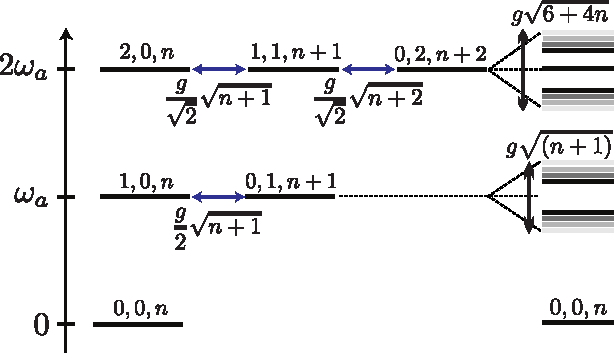
\includegraphics[width=0.7\textwidth]{./figs_Komar2013/fig4a.pdf}\\
%   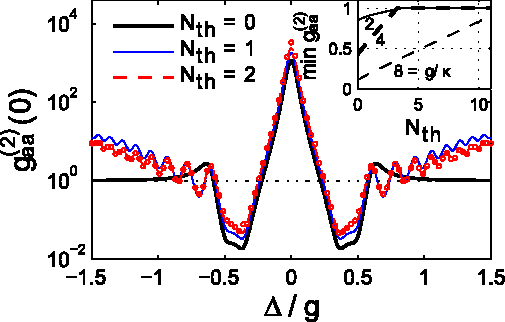
\includegraphics[width=0.7\textwidth]{./figs_Komar2013/fig4b.pdf}\\
%   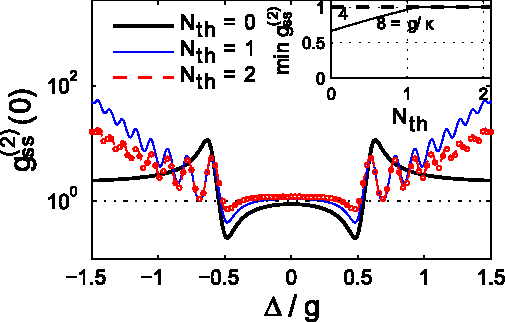
\includegraphics[width=0.7\textwidth]{./figs_Komar2013/fig4c.pdf}
%   \caption{
%   \label{fig:thermal_g2}(Color online)
%   Correlation functions for finite temperature. (a) Level diagram showing the
%   six states populated by the drive from level $|0,0,n\rangle$ (left), 
%   and the associated
%   eigenmodes (right) with $n$-dependent splittings.
%   (b) Driven mode correlation function $g^{(2)}_{aa}(0)$
%   for thermal mechanical occupation $N_{\rm th} = 0,1,2$.
%   Solid lines show the analytic calculation with $\gamma \rightarrow 0$,
%    and  dots show the full numerical results for $N_{\rm th} = 2$ only.
%   The inset shows the minimal $g^{(2)}_{aa}(0)$ as a function of $N_{\rm th}$ 
%   for several
%   coupling strengths. 
%   (c) Same as (b) for the undriven mode correlation function $g^{(2)}_{ss}(0)$. 
%   Parameters are $g/\kappa=20$, and (for numerics) $\gamma/\kappa =  10^{-3}$.
% }
% \end{figure} 
% % ================================== 



%%%%%%%%%%%%%%%%%%%%%%%%%%%%%%%%%%%%%%%%
%%%%%%%%%%%%%%%%%%%%%%%%%%%%%%%%%%%%%%%%
\section{Delayed coincidence and single phonon states}
\label{sect:Delayed_coincidence}


In addition to the equal-time correlations discussed above,
quantum signatures can also be manifested in photon
intensity correlations with a finite time delay.
We now turn to a discussion of  delayed coincidence
characterized by the 
two-time
intensity correlations functions,
\bel
\label{eq:g2_tau}
	g^{(2)}_{ii}(\tau) = \frac{\ev{c_i\+(0) c_i\+ (\tau) c _i(\tau)
	c_i(0)}}{\ev{c_i\+ c_i}^2},
\eel
for both driven and undriven modes, $i = a,s$.
Expressing this correlation in terms of a classical
light intensity $I$,
$g^{(2)}(\tau) = \ev{ I(\tau) I(0) } / \ev{ I }^2$,
and
using the Schwarz inequality, we
obtain the inequalities \cite{Carmichael1991, Brecha1999},
\begin{align}
  \label{eq:classical_criterium}
 	g^{(2)}(\tau) &\leq g^{(2)}(0),	%\quad &(\text{classical}),
	\\
	 |g^{(2)}(\tau)-1| & \leq |g^{(2)}(0)-1| .%\quad &(\text{classical}),
\end{align}
Similar to the classical inequality
$g^{(2)}(0) > 1$ at zero delay, 
violation of either of these inequalites
at finite delay is
a signature of quantum light. 
We calculate the delayed coincidence correlation
functions
for both the driven and undriven modes.


\subsection{Driven mode}
The
correlation function $g^{(2)}_{aa}(\tau)$ is shown in \reffig{fig:g2aatau}(a)
for two values of the detuning $\Delta$.
The most striking feature
is the apparent vanishing of  $g^{(2)}_{aa}(\tau)$
at several values of $\tau$ when the
detuning is $\Delta = 0$ (curve A in \reffig{fig:g2aatau}(a)).
These are due to Rabi oscillations at frequency
$g/2$ following the detection of a photon.
This vanishing of the finite delay correlation function
is reminiscent of  wavefunction collapse that
occurs in a cavity containing an 
atomic ensemble \cite{Carmichael1991},
and while its origins are similar, there are important
differences as we now discuss.




We can understand the finite delay intensity
correlations
in terms of the simple six-level model discussed
in the previous section.
We extend
this model to describe finite delay correlations
by considering the effect of photodetection on
the steady state of the system.
Detection of a photon in the driven mode projects
the system onto the conditional state \cite{QuantumNoise},
\bel
	\label{eq:psi^a}
	\ket{\psi^a} = \frac{c_a \ket{\psi}}{||c_a \ket{\psi} ||},
\eel
where $\ket{\psi}$ is given by \refeq{eq:psi} with steady state amplitudes
and $|| \cdot ||$ denotes normalization after the jump.
The conditional state $\ket{\psi^a}$ has an {\it increased}
amplitude $A_{100}$ after the jump
(see jump at $\tau = 0$ in \reffig{fig:g2aatau} (b)).
Following this initial photodetection, the amplitude 
$A_{100}$
subsequently undergoes Rabi oscillations with frequency $g/2$,
and decays back to its steady state at rate $2\kappa$. 
For sufficiently large bunching at zero delay and
strong coupling $g > \kappa$, the  Rabi oscillations of the amplitude
$A_{100}(\tau)$ can cause it to cross zero 
several times before it decays back
to steady state.
As the probability to detect a second photon is dominated by $A_{100}$,
its zeros are responsible for the zeros in the correlation
function $g^{(2)}_{aa}(\tau)$ zero at these delay times.





The zeros in $g^{(2)}(\tau)$ appear similar
to those exhibited  in
a cavity strongly coupled to
an atomic ensemble \cite{Carmichael1991, Rice1988, Brecha1999} or a single atom
\cite{Chang2007}. 
However, in stark contrast to the atomic case,
the zeros in \reffig{fig:g2aatau}(a)
are the result of Rabi oscillations  following
the initial quantum jump.
This is qualitatively different from
the atomic case, where the change in
sign of the relevant amplitude (the analogy of $A_{100}$)
occurs {\it immediately} after the jump itself, and the amplitude
is damped back to steady state at the atomic
decay rate $\Gamma$, without Rabi oscillation. 
As a consequence, the vanishing correlation
function in the atomic case occurs
at a delay set by $\tau_0 \sim \gamma^{-1}\ln C$, 
requiring only strong cooperativity $C = g^2/ \kappa \gamma > 1$
to be visible.
On the other hand,
the zeros in \reffig{fig:g2aatau}(a)
occur at delay times set by  $\tau \sim 1/g$,
requiring strictly strong coupling $g > \kappa$.








Before moving on to correlations of the undriven mode,
we briefly discuss the correlations of the driven mode at the
 other value of  detuning shown in 
\reffig{fig:g2aatau}(a).
 At detuning
$\Delta = \frac{g}{\sqrt{2}}$ (curve E),
which shows bunching at zero time,
$g^{(2)}_{aa}(0) \gtrsim 1$, 
increases  above its initial value at
finite delay.
This is a violation of the classical inequality in
\refeq{eq:classical_criterium}, 
and is an example of ``delayed bunching,"
or an increased probability to detect a second
photon at a finite delay time.
A similar effect was recently studied
in a single mode OMS \cite{Kronwald2012}.
However, like the Rabi oscillations,
the increased correlation function decays back to its steady state
value of 1 on
the timescale of $\kappa^{-1}$.
%%%%%%%%%%%%%%%%%%%%%%%%%%%%%
%%%%%%%%%%%%%%%%%%%%%%%%%%%%%
\begin{figure} 
\centering
  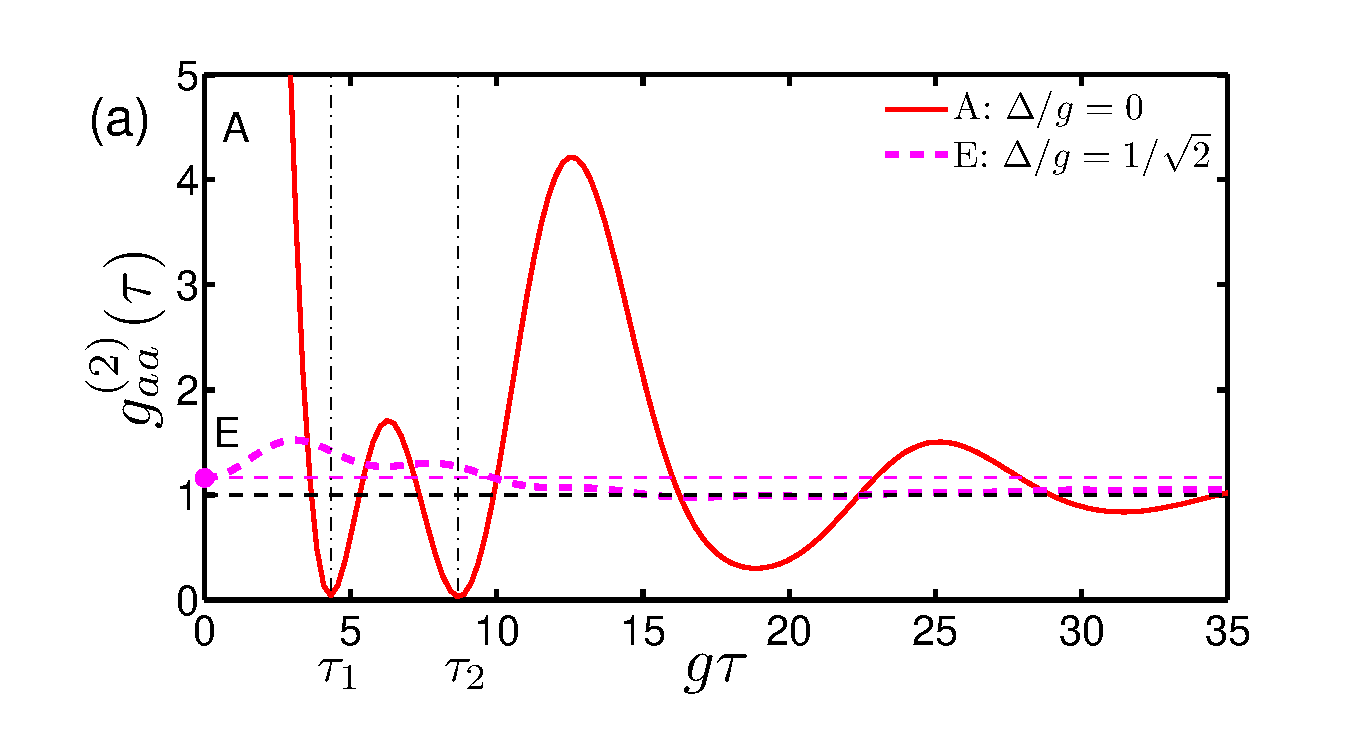
\includegraphics[width=0.9\textwidth]{./figs_Komar2013/fig5a.pdf}\\[-0.5cm]
  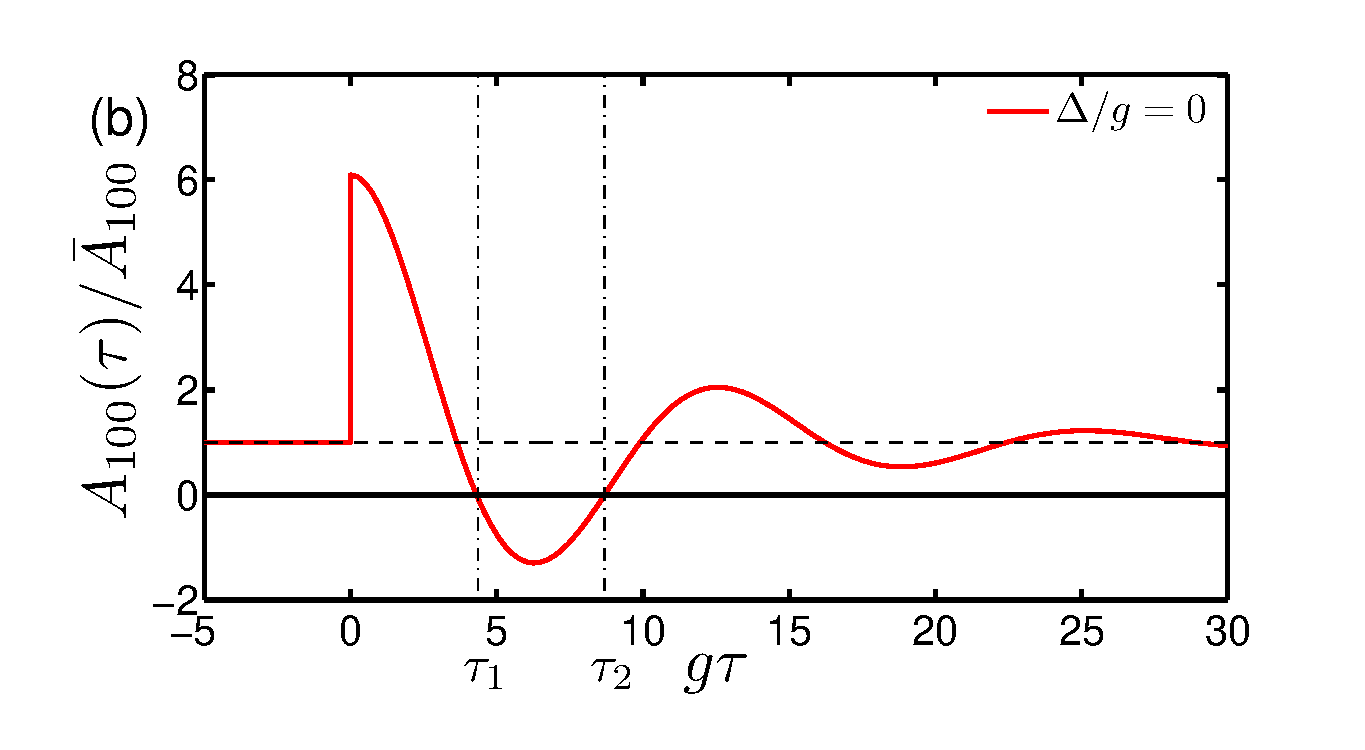
\includegraphics[width=0.9\textwidth]{./figs_Komar2013/fig5b.pdf}
  \caption
  [Autocorrelation of mode $a$]
  {
  \label{fig:g2aatau}
  (a) Finite time delay intensity
  correlation function $g^{(2)}_{aa}(\tau)$  for detunings
  $\Delta/g = 0 \text{ (A)}$ and $\frac{1}{\sqrt{2}}
  \text{ (E)}$.
  Detuning for curve A is the same as marked in \reffig{fig:spectrum_a},
  while E shows a new effect not seen at equal times.
  Thin dashed line indicates the classical bound 
  (see \refeq{eq:classical_criterium}) for curve E. 
  (b) Evolution of amplitude $A_{100}$ (normalized by its
  steady state value)
  at detuning A, $\Delta/g = 0$,
  after detecting a driven $c_a$ photon at $\tau = 0$. 
  Vertical dash-dotted lines mark delay times ($\tau_1, \tau_2$) where this amplitude
  vanishes resulting in the vanishing of $g^{(2)}_{aa}(\tau)$
  in (a).
  Parameters are $g/\kappa = 8$ and $\gamma/\kappa$ = 0.02. 
  } 
\end{figure}
%%%%%%%%%%%%%%%%%%%%%%%%%%%%%
%%%%%%%%%%%%%%%%%%%%%%%%%%%%%




\subsection{Heralded single phonon states}

We now turn to a discussion of the delayed coincidence
correlations of the undriven mode $c_s$.
We note that correlations of the driven
and undriven modes can be measured separately
provided sufficient frequency resolution, smaller than
  the mechanical frequency.
The correlation function
$g^{(2)}_{ss}(\tau)$
of the undriven mode
is shown in \reffig{fig:g2sstau} for several
values of detuning.
Similar to the driven mode, the
correlation function of the undriven mode
exhibits Rabi oscillations 
that decay on the short optical
timescale
$1/\kappa$.
For detuning $\Delta = 0$ and 
$\Delta/g = \frac{\sqrt{6}}{4}$
(curves A and D in \reffig{fig:g2sstau}),
the correlation $g^{(2)}_{ss}(\tau)$
is described by
our previous six-level 
model of Eqs. (\ref{eq:c000}--\ref{eq:c022}).
However,  at detuning $\Delta = \frac{g}{\sqrt{2}}$
(curve E), we see that
$g^{(2)}_{ss}(\tau)$ has a long
tail that decays
on the much longer mechanical timescale $1/\gamma$.
This is due to the heralded preparation
of a single phonon by detection of a photon in the
undriven mode, as we now discuss.
%and can be understood
%by a simple extension of the six-level model
%discussed above.
%%%%%%%%%%%%%%%%%%%%%%%%%%%%%
%%%%%%%%%%%%%%%%%%%%%%%%%%%%% 
\begin{figure}[htb] \centering
  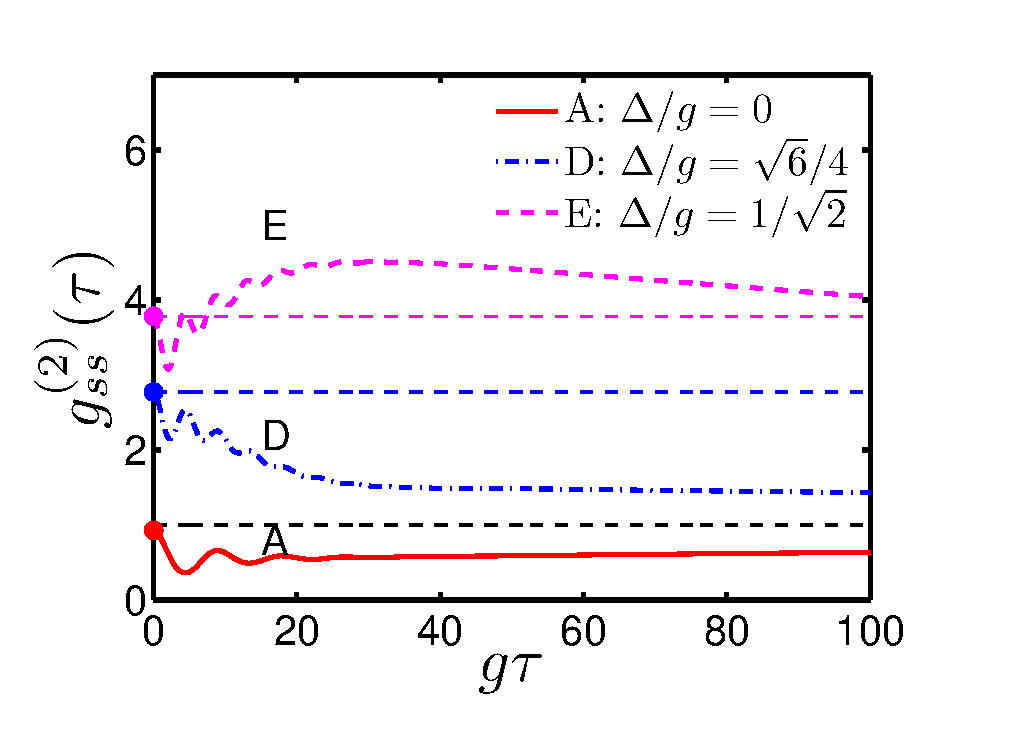
\includegraphics[width=0.8\textwidth]{./figs_Komar2013/fig6.pdf}
  \caption[Autocorrelation of mode $s$]
  {
  \label{fig:g2sstau}
  Finite time delay intensity correlation function $g^{(2)}_{ss}(\tau)$
  for detunings $\Delta/g = 0 \text{ (A)}, \sqrt{6}/4 \text{ (D)}$
  and
  $\frac{1}{\sqrt{2}} \text{ (E)}$.
  Thin dashed lines indicate the classical bounds
  (see  \refeq{eq:classical_criterium}).
  Labels A, D, E correspond to the same detunings
  marked in 
  \reffig{fig:spectrum_a}
  and
  \reffig{fig:g2aatau}.
  Parameters are $g/\kappa = 8$, and $\gamma/\kappa$ = 0.02.
  }
\end{figure}
%%%%%%%%%%%%%%%%%%%%%%%%%%%%%
%%%%%%%%%%%%%%%%%%%%%%%%%%%%%



The increase in delayed coincidence can be understood
by extending the above analytic six-level model to account
for the conditional state of the system after detection
of a photon in the undriven mode.
To do this,
we simply add three additional states to
the six-level ansatz in  \refeq{eq:psi},
\bel
\label{eq:psi9}
	\ket{\psi} = \dots + A_{001}\ket{001} + A_{101}\ket{101} + A_{012}\ket{012},
\eel
since these are the states populated by detection
of a $c_s$ photon from the original six states (see \reffig{fig:levels_jumps}).
Using the same 
%non-Hermitian dynamics
approach as before, we obtain the following equations for the
amplitudes,
\bal
	\label{eq:c001}
	\dot A_{001} &\approx& -\frac{\gamma}{2}A_{001},\\[0.2cm]
	\dot A_{101} &=& -i\frac{g}{\sqrt{2}} A_{012} -i\Omega A_{001} -
	\tilde\kappa A_{101},\\
	\label{eq:c012}
	\dot A_{012} &=& -i\frac{g}{\sqrt{2}} A_{101} - \tilde\kappa A_{012},
\eal
where we used $\gamma \ll \kappa$ and
kept the leading term in \refeq{eq:c001}.
We obtain $g^{(2)}_{ss}(\tau)$
by solving these equations for initial
conditions determined by the conditional state $\ket{\psi^s}$
after a quantum jump, 
\bel
	\label{eq:psi^s}
	\ket{\psi^s} = \frac{c_s \ket{\psi}}{||c_s \ket{\psi}||},
\eel
which is a superposition of states $\ket{001}, \ket{101}, \ket{012}$
(see Appendix \ref{sect:App:steady_state} 
%\ref{sect:two-time_analytic} 
for details), but in the limit of weak driving consist mainly of $|001\rangle$. 


Detection of a photon in the undriven mode
implies that the three-wave mixing interaction
converted a photon from the driven mode into
the undriven mode by simultaneously adding a phonon.
The relevant three-level subspace after the jump 
(see \reffig{fig:levels_jumps}) has a similar structure as in the steady state, 
but the presence of an extra phonon
modifies the splitting of the one-photon 
states $|1^\prime_{\pm}\rangle=(|101\rangle \pm |012\rangle)/\sqrt{2}$  to
$\frac{g}{\sqrt{2}}$ 
(instead of $g/2$ without a phonon).
%
%The increase in delayed coincidence
%at specific laser detuning is a direct consequence
%of this conversion,
%as illustrated in \reffig{fig:levels_jumps}.
%In steady state, the system occupies the
%six levels of \refeq{eq:psi}, shown 
%on the left in \reffig{fig:levels_jumps}.
%After detection of an undriven $c_s$ photon,
%the 
%emitted  phonon slowly decays back
%to its ground state at rate $\gamma$, 
%during which time the system is in the conditional
%subspace shown on the
%right in \reffig{fig:levels_jumps}.
%%%%%%%%%%%%%%%%%%%%%%%%%%%%%
%%%%%%%%%%%%%%%%%%%%%%%%%%%%% 
\begin{figure}[htb]
\centering  
  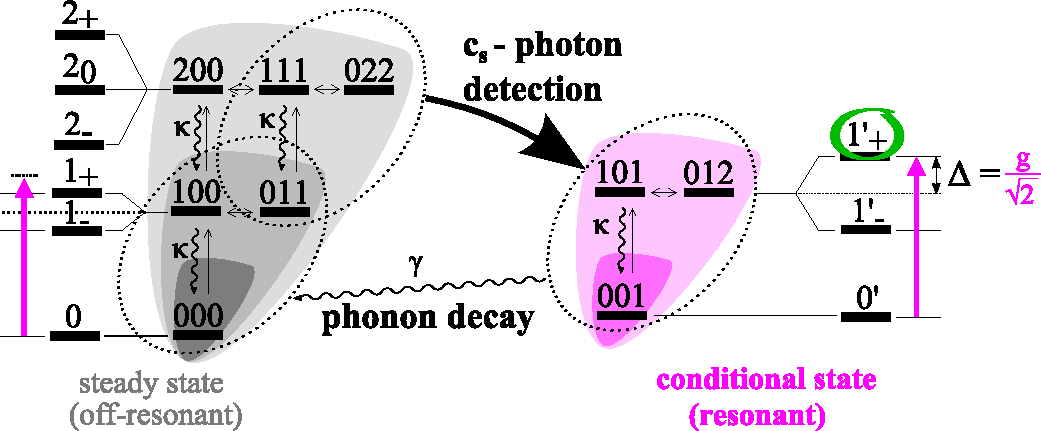
\includegraphics[width=0.85\textwidth]{./figs_Komar2013/fig7.pdf}\\
  \caption[Diagram with metastable subspace]
  {
  \label{fig:levels_jumps}
  Effect of detection of a $c_s$ photon
  at detuning E ($\Delta/g = \frac{1}{\sqrt{2}}$).
  In steady state (gray region on left), 
  the drive is far off-resonant.
  However, after detection of a $c_s$ photon the system
  jumps into the conditional subspace (pink region on right).
  Due to the presence of an extra phonon in this subspace,
  the drive is resonant and the probability to detect a second
  photon is much higher than in steady state.
  This increased probability persists
  as long as the extra phonon,
  which decays slowly at rate $\gamma$.
  }
\end{figure}
%%%%%%%%%%%%%%%%%%%%%%%%%%%%%
%%%%%%%%%%%%%%%%%%%%%%%%%%%%%
This changes
the one-photon resonance condition
for the drive to $\Delta = \frac{g}{\sqrt{2}}$.
Therefore, at this value of the detuning,
the process of
exciting the system and emitting a single $c_s$ photon
is off-resonant;
while after the detection of a first $c_s$ photon
the system is prepared in $|001\rangle$, bringing
it into resonance with the drive.
%brings the system into resonance with the drive,
This {\it enhances}
the probability for subsequent excitation and emission
of a second $c_s$ photon, increasing
the correlation function at finite delay.
%successive excitation of the second photon 
%occurs exactly on resonance. 
%while 
%resonant in the presence of an extra phonon,
%such that 
%the probability to detect a second 
%photon 
%This process {\it enhances} the probability 
%of photon coincidences in the undriven mode, 
The maximum delayed coincidence
occurs after a delay of $\tau \sim 1/\kappa$,
when the photons have reached the
metastable steady state
in the conditional  subspace with one 
extra phonon.
Eventually, the delayed coincidence
returns to its true steady state value
of one
%of $g^{(2)}_{ss}(\tau) \rightarrow 1$
on the timescale
$\tau \sim 1/\gamma$, which is the mechanical decay time of the
state $|001\rangle$. 
%\pk{Detuning $\Delta/g = 1/\sqrt{2}$ is chosen in order
%to optimize the visibility of the long tail of $g^{(2)}_{ss}$. 
The long tails
observed for other values of detuning (curves A and D) are
also
due to the presence of an extra phonon,
but in these cases the system remains off-resonant
after the initial $c_s$ photon and the effect is less
 pronounced.
Note that the
probability  to detect a photon from the {\it driven} mode also increases in 
the conditional state, so a similar effect is seen in the delayed 
cross-correlation function $g^{(2)}_{as}(\tau)$, where the photon in the 
undriven mode is detected first.

%Detection of a photon in the undriven mode
%implies that the three-wave mixing interaction
%converted a photon in the driven mode into
%one in the undriven mode by generating a phonon.
%After this first detection, the 
%emitted single phonon slowly decays back
%to its ground state at rate $\gamma$.
%During this slow decay, the presence
%of the extra phonon modifies the resonance
%condition of the coupled OM system, 
%changing the probability to detect a second photon.
%Specifically, if the drive detuning is chosen so that the
%system is off-resonant in steady state
%(at zero temperature), but
%resonant in the presence of an extra phonon,
%then 
%the probability to detect a second 
%photon {\it increases}
%after detection of a photon in the undriven mode.
%This increase in the  coincidence correlation
%at finite delay seen in 
%$g^{(2)}_{ss}(\tau)$
%violates the classical inequality in
%\refeq{eq:classical_criterium}.



%%%%%%%%%%%%%%%%%%%%%%%%%%%%%%%%%%%%%%%%
%%%%%%%%%%%%%%%%%%%%%%%%%%%%%%%%%%%%%%%%
\section{Reaching strong coupling}
\label{sect:Experimental values}


The nonclassical correlations predicted in this paper 
require  strong optomechanical coupling, $g > \kappa$, 
as well as sideband resolution, $\omega_m \gg \kappa,\gamma$. 
While the combination of these conditions has not 
yet been demonstrated, 
several experimental efforts 
%in OMSs 
are currently 
directed at reaching this regime. 
By using micro- and nano-fabricated OMSs such 
as microtoroids or photonic crystal beams, 
high frequency mechanical systems  with 
$\omega_m\approx 50$ MHz - 5 GHz can be combined 
with low loss optical modes, such that the 
condition $\omega_m \gg \kappa \gg \gamma$ is satisfied
\cite{Safavi-Naeini2011a, Schliesser2008, Eichenfield2009}.
At the same time the mechanical system can already 
be prepared close to the quantum ground state by working at cryogenic temperatures. 
In micro-fabricated OMSs, single-photon couplings of 
about $g/\kappa \approx 0.001$ have been demonstrated 
\cite{Eichenfield2009, Ding2011,Verhagen2011}
%\cite{Teufel2011,Teufel2011a}.
The largest value to date of $g/\kappa \approx 0.007$ 
has been reached in photonic crystal beam
resonators \cite{Chan2012}, where
colocalized optical and vibrational resonances are
highly confined to maximize coupling
while the surrounding structure is engineered  
to minimize loss.
Conversely, in cold atomic experiments
the effective strong OM coupling regime has been
reached \cite{Purdy2010}, while sideband resolution remains
a challenge \cite{Stamper-kurn}. 


%In experiments with a 
%micromechanical membrane capacitively coupled to
%a superconducting resonant microwave circuit,
%a ratio of $g/\kappa \approx 0.001$
%has been achieved \cite{Teufel2011,Teufel2011a}.
%The strongest
%ratio to date of ($g/\kappa \approx 0.005$) were 
%reached in photonic crystal beam
%resonators \cite{Chan2012}, where
%colocalized optical and vibrational resonances are
%highly confined to maximize coupling
%while the surrounding structure is engineered
%to minimize loss.
%However in systems with the highest achieved
%ratio of $g/\kappa$, two orders of magnitude
%improvement is required to reach
%the strong coupling
%regime. 


There are several existing
proposals for how to meet the challenge
of $g/\kappa > 1$ 
in the photonic crystal beam setup.
First, 
the single-photon optomechanical coupling can 
be increased by making use of
nanoslots in the structure \cite{Robinson2005, Davanc2012} 
to further localize the electric field at 
the position of the mechanical mode.
This could improve $g$ by a factor of 10
\cite{Ludwig2012}.
Second, numerical studies 
suggest that $\kappa$ can be further decreased
by fine tuning the size and position of the slots in
the photonic crystals \cite{Notomi2008,Tanaka2008}. 
Finally, new materials are currently being tested for an 
overall improvement of the OM properties of nano-fabriquated devices \cite{Xiong2012}.
Thus by using these ultrahigh $Q$ photonic crystals or 
similar designs, an increase of $g/\kappa$ by a factor of $\sim 100$ 
is realistic. 
Note that once the strong coupling condition has been achieved, 
the implementation of two or multimode OMSs 
with adjustable tunneling $2J\sim \omega_m$ can be realized via evanescent field
coupling, as has already been demonstrated in the weak coupling regime
\cite{Safavi-Naeini2011a, Eichenfield2009, Grudinin2010}.


%Implementing these
%proposals in experiment will clearly be challenging;
%however, we stress that 
%a two-mode approach can remove dependence upon the much larger
%mechanical frequency $\omega_m \gg \kappa$, making the realization of these
%feasible.




%%%%%%%%%%%%%%%%%%%%%%%%%%%%%%%%%%%%%%%%
%%%%%%%%%%%%%%%%%%%%%%%%%%%%%%%%%%%%%%%%
\section{Conclusions}
\label{sect:Conclusion}

We have studied  nonclassical intensity correlations in a
driven, near-resonant 
optomechanical system with  one mechanical and two optical modes.
In the regime of strong coupling $g > \kappa$, this system
allows for nonlinear quantum optics through a resonant three-mode 
interaction in which the exchange of two photons is mediated by a phonon.
We have identified several different processes
that can lead to nonclassical antibunching and delayed bunching, 
and we have  
derived a simple analytic model that allows us to 
describe and interpret photon-photon correlations in this 
system both at zero and at finite temperature. 
Our findings will be important as experiments
approach the regime of strong 
OM coupling, and for potential applications of 
OMSs for quantum information processing. 
%
%The requirement of strict strong coupling
%is in contrast to analogous atom-cavity
%systems, in which nonclassical correlations 
%persist in the less stringent regime of 
%strong cooperativity $g^2 > \kappa\gamma$.
%This is not surprising, since all states with appreciable population
%in steady state involve photons, which decay at rate $\kappa$.
%Nonetheless, 
In particular, the long-lived
correlation found for the undriven mode 
raises the intriguing possibility to
exploit such a setup as a quantum memory.
The generation of
heralded single phonons on detection
of a photon from the undriven mode may have implications
for building OM quantum 
repeaters and quantum communication devices.


%%%%%%%%%%%%%%%%%%%%%%%%%%%%%%%%%%%%%%%%
%%%%%%%%%%%%%%%%%%%%%%%%%%%%%%%%%%%%%%%%



